%--------------------------------------------------
\subsection{Prototipo 3: Integración con servicios REST a panel de administración}

%--------------------------------------------------
\subsubsection{Análisis}

Dentro de este prototipo se satisface los requerimientos funcionales \hyperlink{RFPA}{Iniciar sesión},\hyperlink{RFPA}{Visualizar información de anuncios publicados} y \hyperlink{RFPA}{Visualizar información de Beacons} definidos previamente en el capítulo del ``Bosquejo general de la aplicación''  con el título de ``Requerimientos funcionales del Panel de Administración''. \\ \par

\title{\textbf{Diagrama de casos de uso \\}}
En la figura \ref{casosusomiddleware2} se puede visualizar el diagrama de casos de uso actualizado. \\
Modificaciones realizadas: 
\begin{itemize}
\item Se agregó el caso de uso \textbf{Cerrar sesión} al diagrama.
\item Se agregó el caso de uso \textbf{CUPA5.1:Publicar anuncio}
\item Se cambió el caso de uso \textbf{CUPA5.1}  del prototipo 2 a \textbf{CUPA5.1.2:Añadir departamento(s)}
\item Se cambió el caso de uso  \textbf{CUPA5.2} del prototipo 2 a \textbf{CUPA5.1.1:Añadir producto(s)}
\end{itemize}
 
\FloatBarrier
\begin{figure}[htbp!]
		\centering
			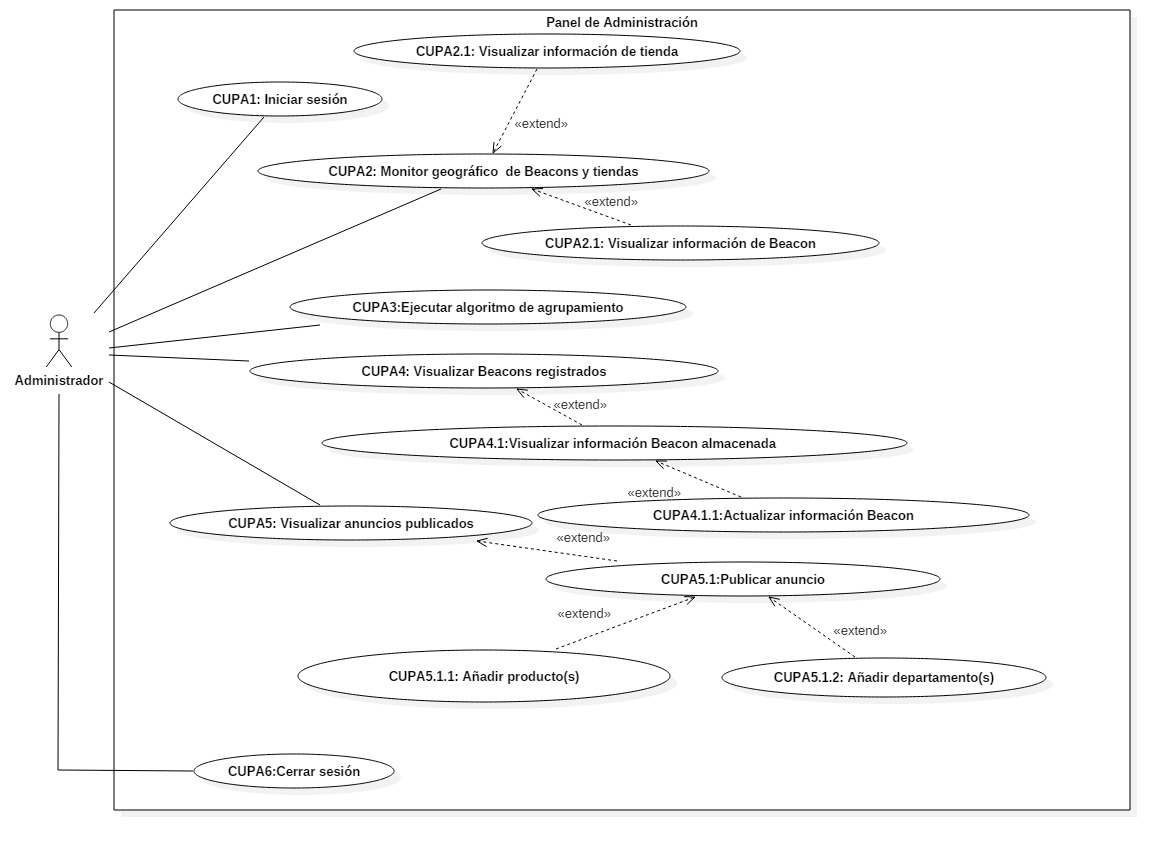
\includegraphics[width=1.1 \textwidth]{imagenes/CU/middleware2}
		\caption{Diagrama de casos de uso.}
		\label{casosusomiddleware2}
\end{figure}
\FloatBarrier


%--------------------------------------------------
\subsubsection{Diseño}
\title{\textbf{Diagramas de secuencia \\}}
La figura \ref{PADS:iniciarsesion} muestra el diagrama satisface el caso de uso \hyperlink{casosdeusoPA}{Iniciar sesión} que se muestra en el diagrama de casos de uso de el primer prototipo. \\
\FloatBarrier
\begin{figure}[htbp!]
		\centering
			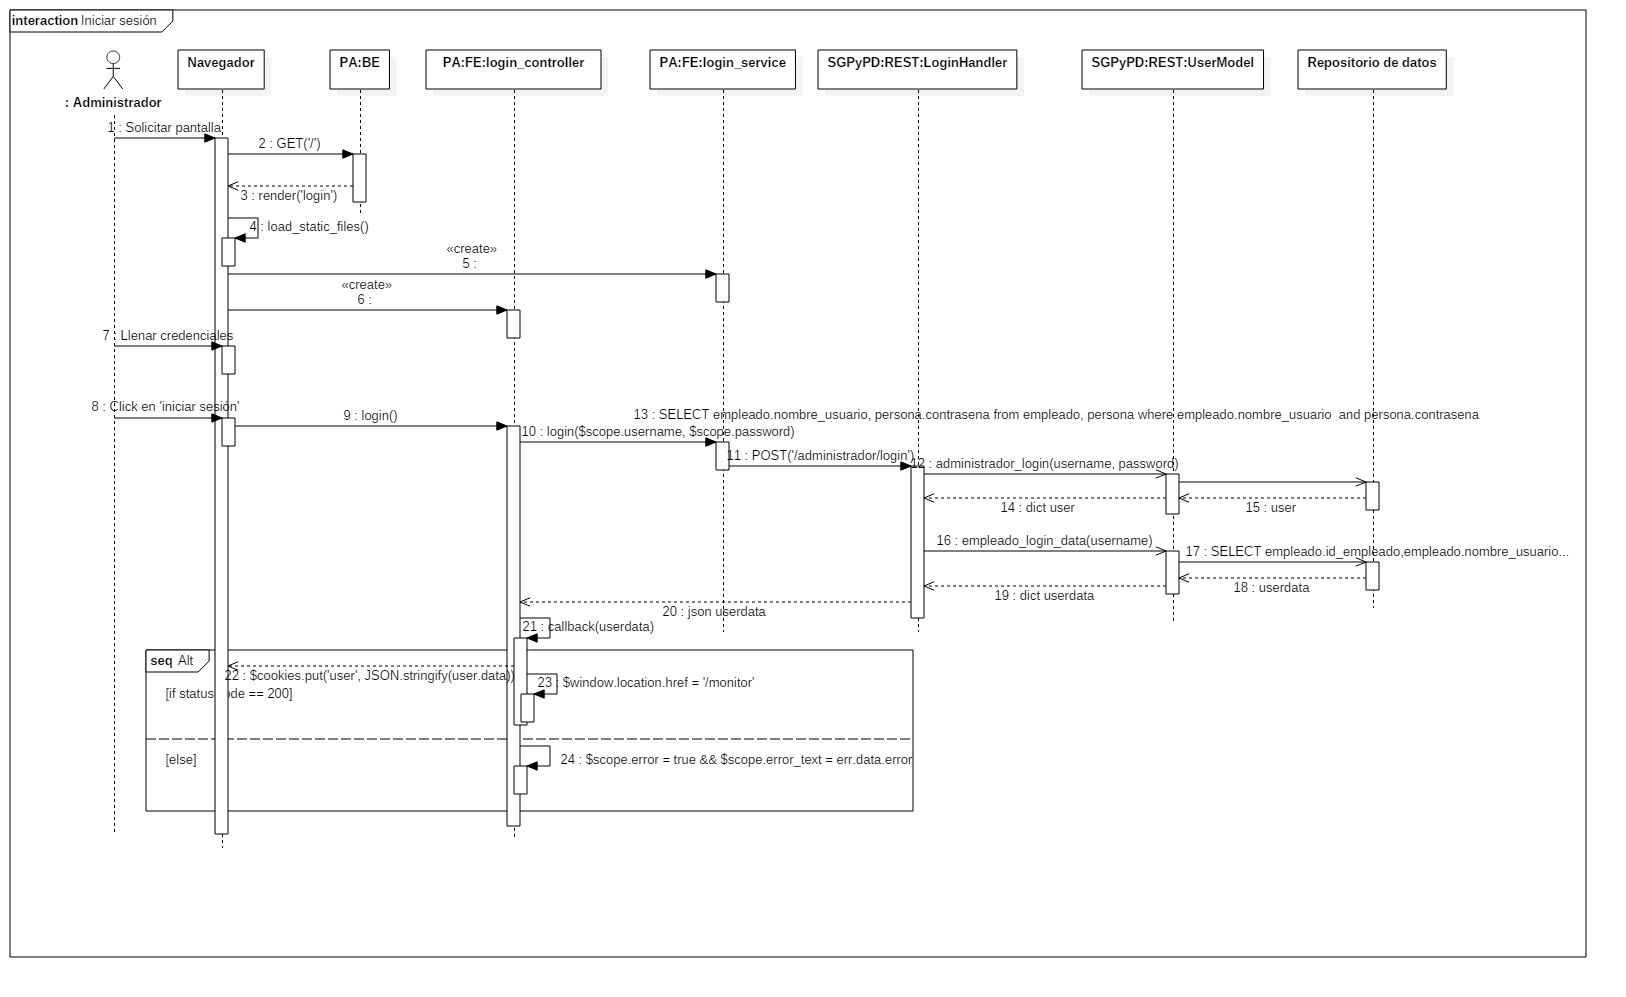
\includegraphics[width=1.1 \textwidth]{imagenes/DSRuben/PA_iniciarsesion}
		\caption{Diagrama de secuencia Iniciar sesión.}
		\label{PADS:iniciarsesion}
\end{figure}
\FloatBarrier


La figura \ref{PADS:cerrarSesion} muestra el diagrama satisface el caso de uso \hyperlink{casosdeusoPA}{Cerrar sesión} que se muestra en el diagrama de casos de uso del prototipo en cuestión. \\
\FloatBarrier
\begin{figure}[htbp!]
		\centering
			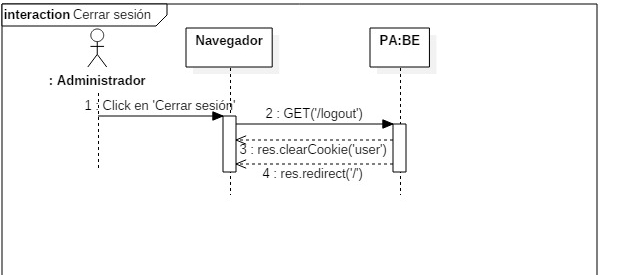
\includegraphics[width=1 \textwidth]{imagenes/DSRuben/PA_cerrarsesion}
		\caption{Diagrama de secuencia Cerrar sesión.}
		\label{PADS:cerrarSesion}
\end{figure}
\FloatBarrier

La figura \ref{PADS:VisualizarBeacon} muestra el diagrama satisface el caso de uso \hyperlink{casosdeusoPA}{Visualizar anuncios publicados} que se muestra en el diagrama de casos de uso. \\
\textit{Notas:}
\begin{enumerate}
\item \textit{El diagrama fue separado en varias figuras para su visualización (Figura \ref{PADS:VisualizarAnuncio}, Figura \ref{PADS:VisualizarAnuncio1}, Figura \ref{PADS:VisualizarAnuncio2}, Figura \ref{PADS:VisualizarAnuncio3}, Figura \ref{PADS:VisualizarAnuncio4}).}
\item \textit{Dentro del diagrama se encuentran también los casos de uso \hyperlink{casosdeusoPA}{Publicar anuncio}, \hyperlink{casosdeusoPA}{Añadir departamento(s)}, \hyperlink{casosdeusoPA}{Añadir producto(s)}} 
\end{enumerate}
\FloatBarrier
\begin{figure}[htbp!]
		\centering
			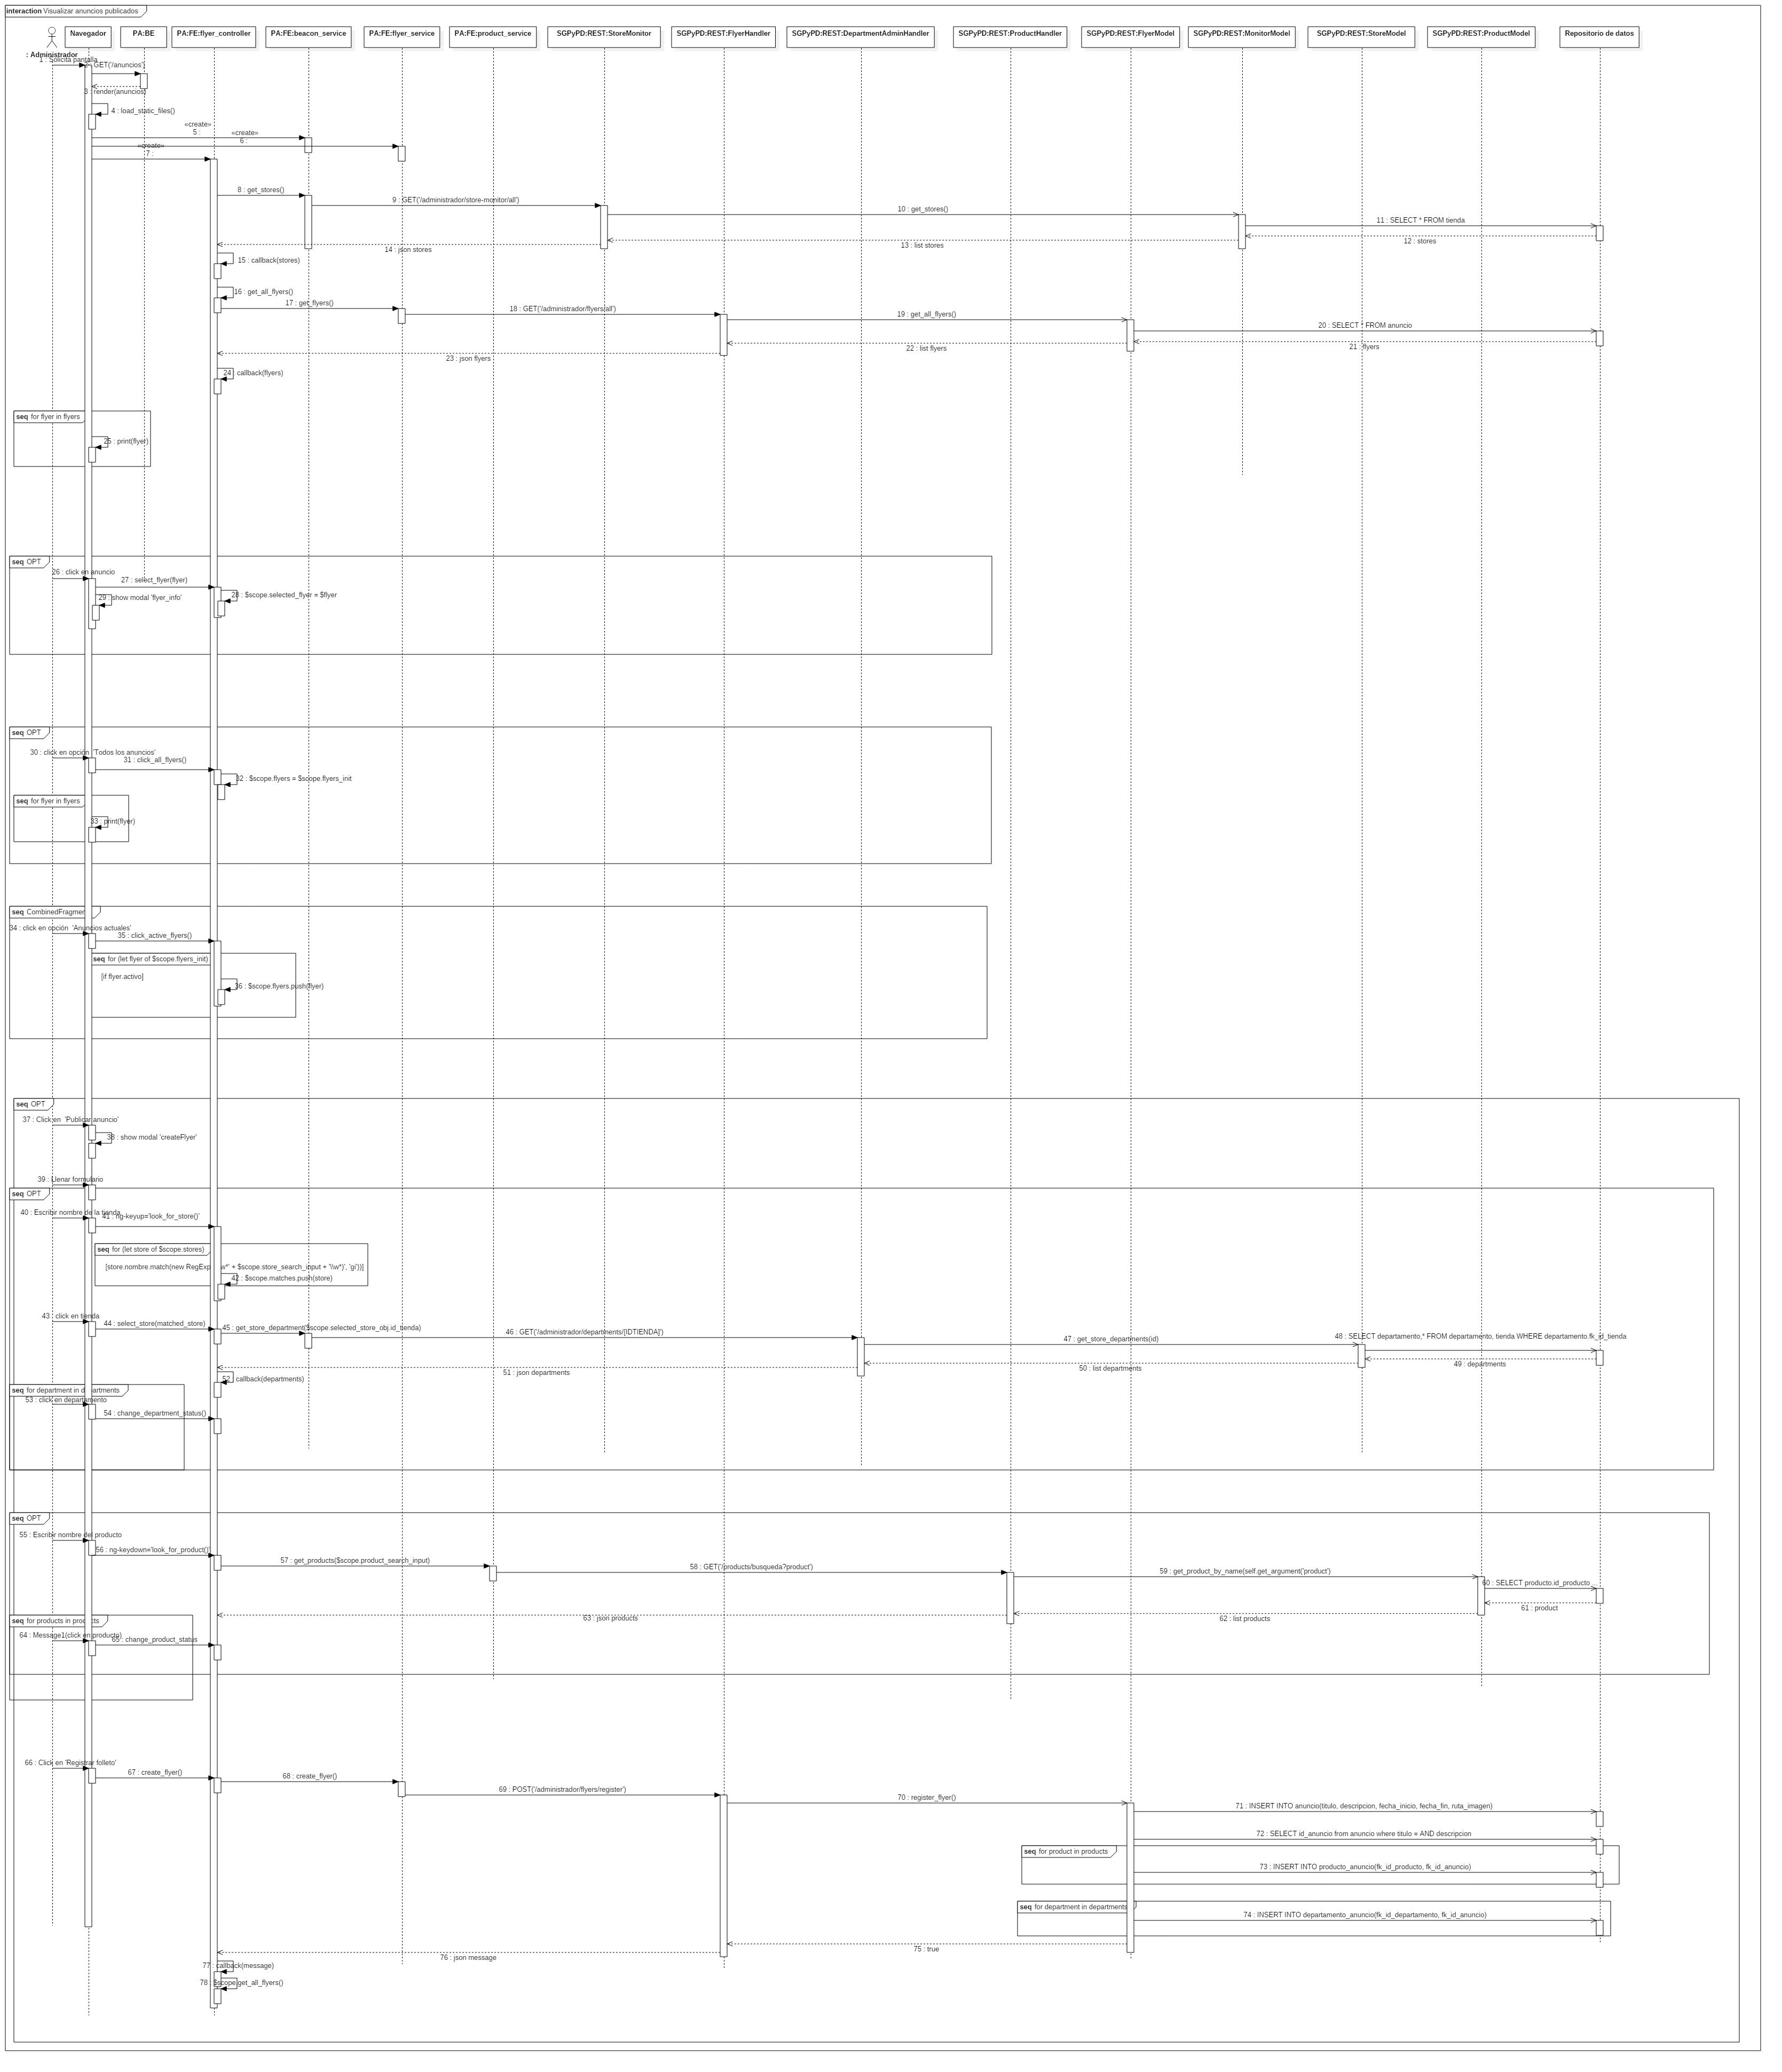
\includegraphics[width=1 \textwidth]{imagenes/DSRuben/anuncios}
		\caption{Diagrama de secuencia Visualizar anuncios publicados (Visualización completa).}
		\label{PADS:VisualizarAnuncio}
\end{figure}
\FloatBarrier

\FloatBarrier
\begin{figure}[htbp!]
		\centering
			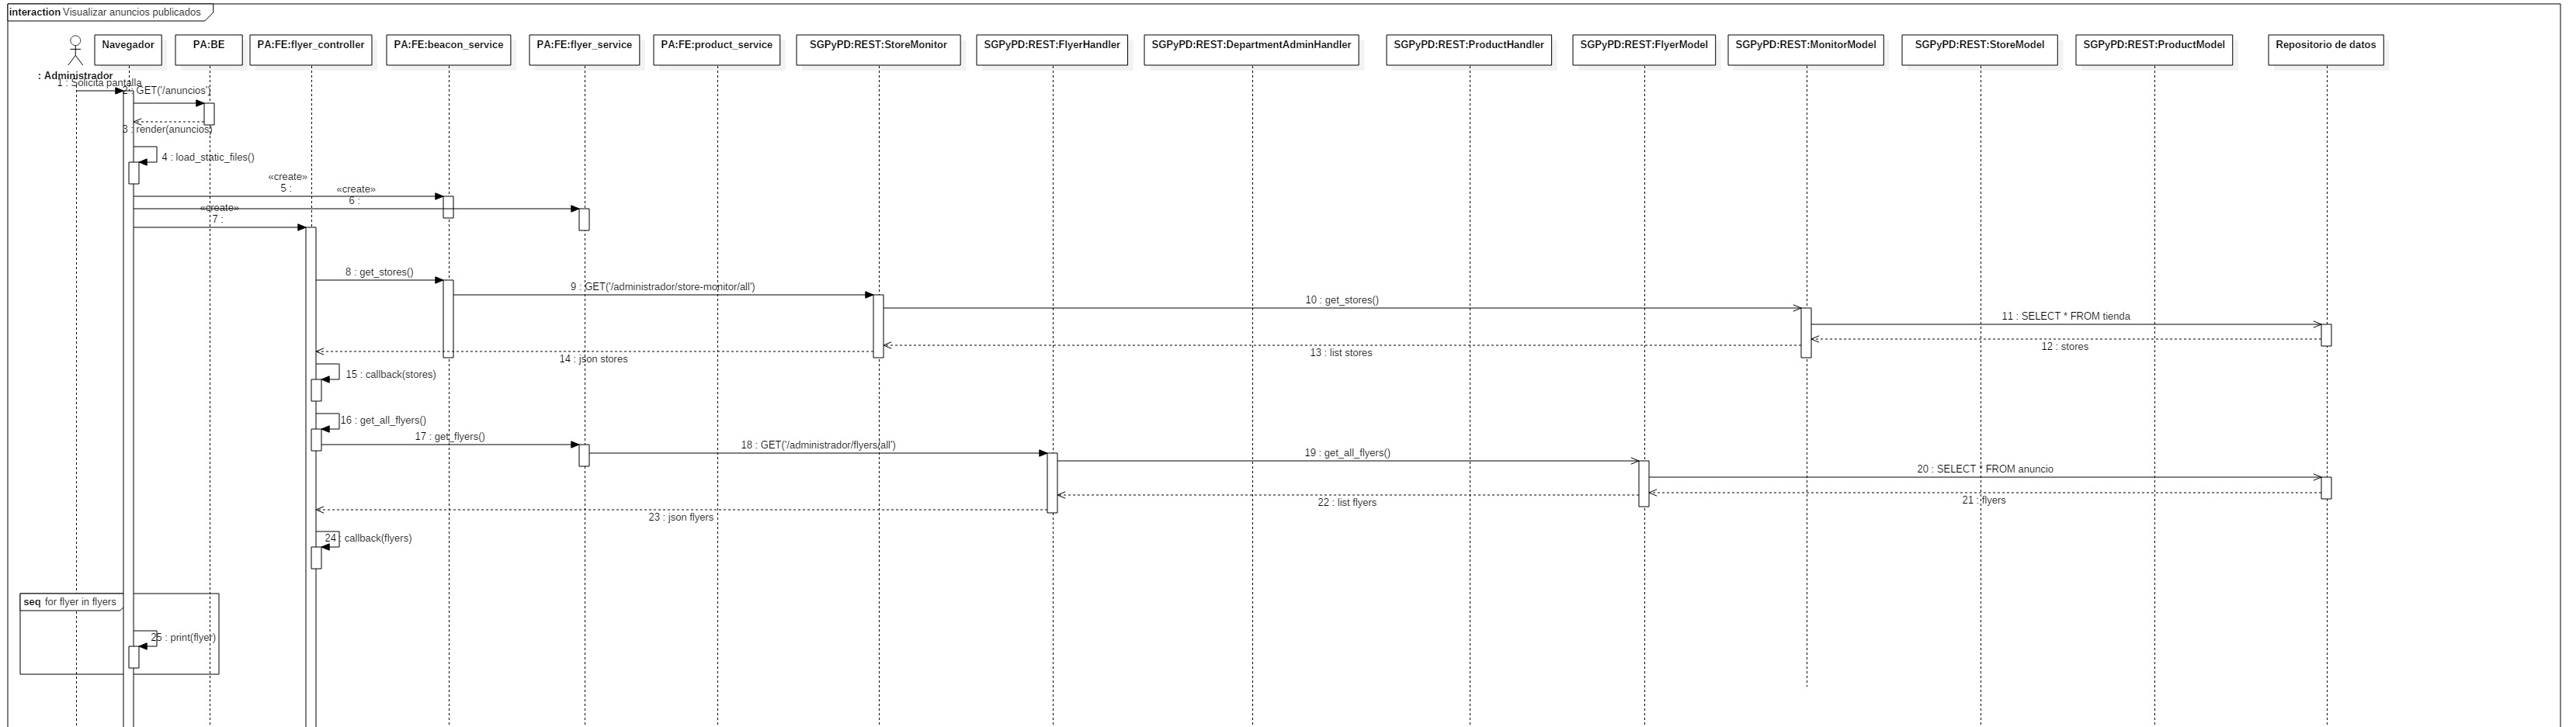
\includegraphics[width=1 \textwidth]{imagenes/DSRuben/anuncios1}
		\caption{Diagrama de secuencia Visualizar anuncios publicados (Parte 1).}
		\label{PADS:VisualizarAnuncio1}
\end{figure}
\FloatBarrier

\FloatBarrier
\begin{figure}[htbp!]
		\centering
			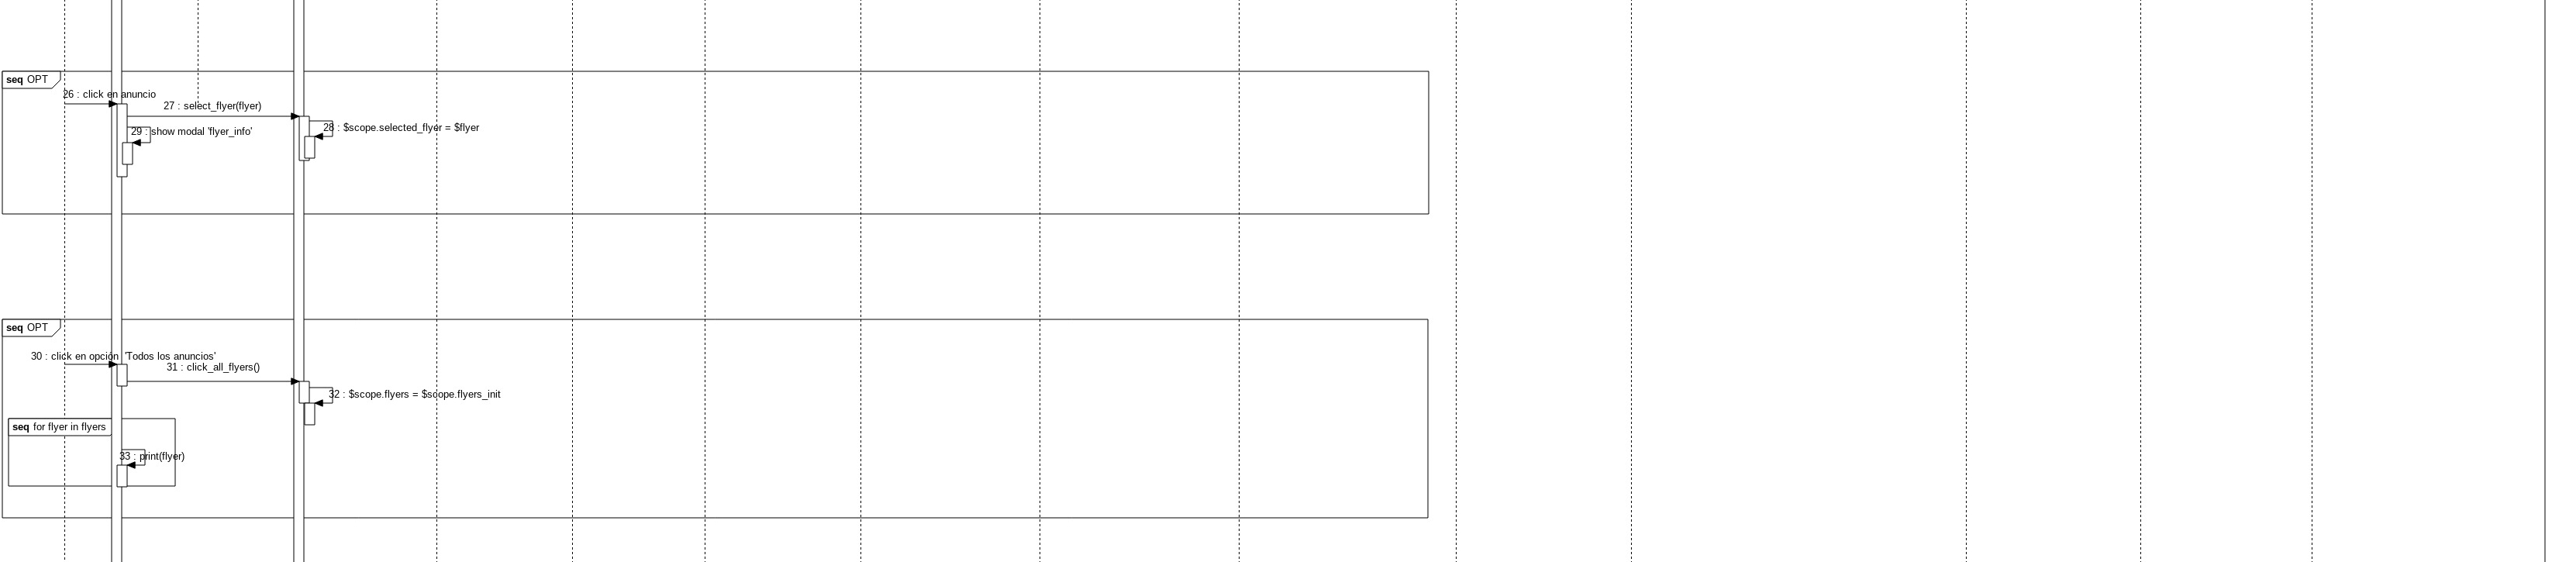
\includegraphics[width=1 \textwidth]{imagenes/DSRuben/anuncios2}
		\caption{Diagrama de secuencia Visualizar anuncios publicados (Parte 2).}
		\label{PADS:VisualizarAnuncio2}
\end{figure}
\FloatBarrier

\FloatBarrier
\begin{figure}[htbp!]
		\centering
			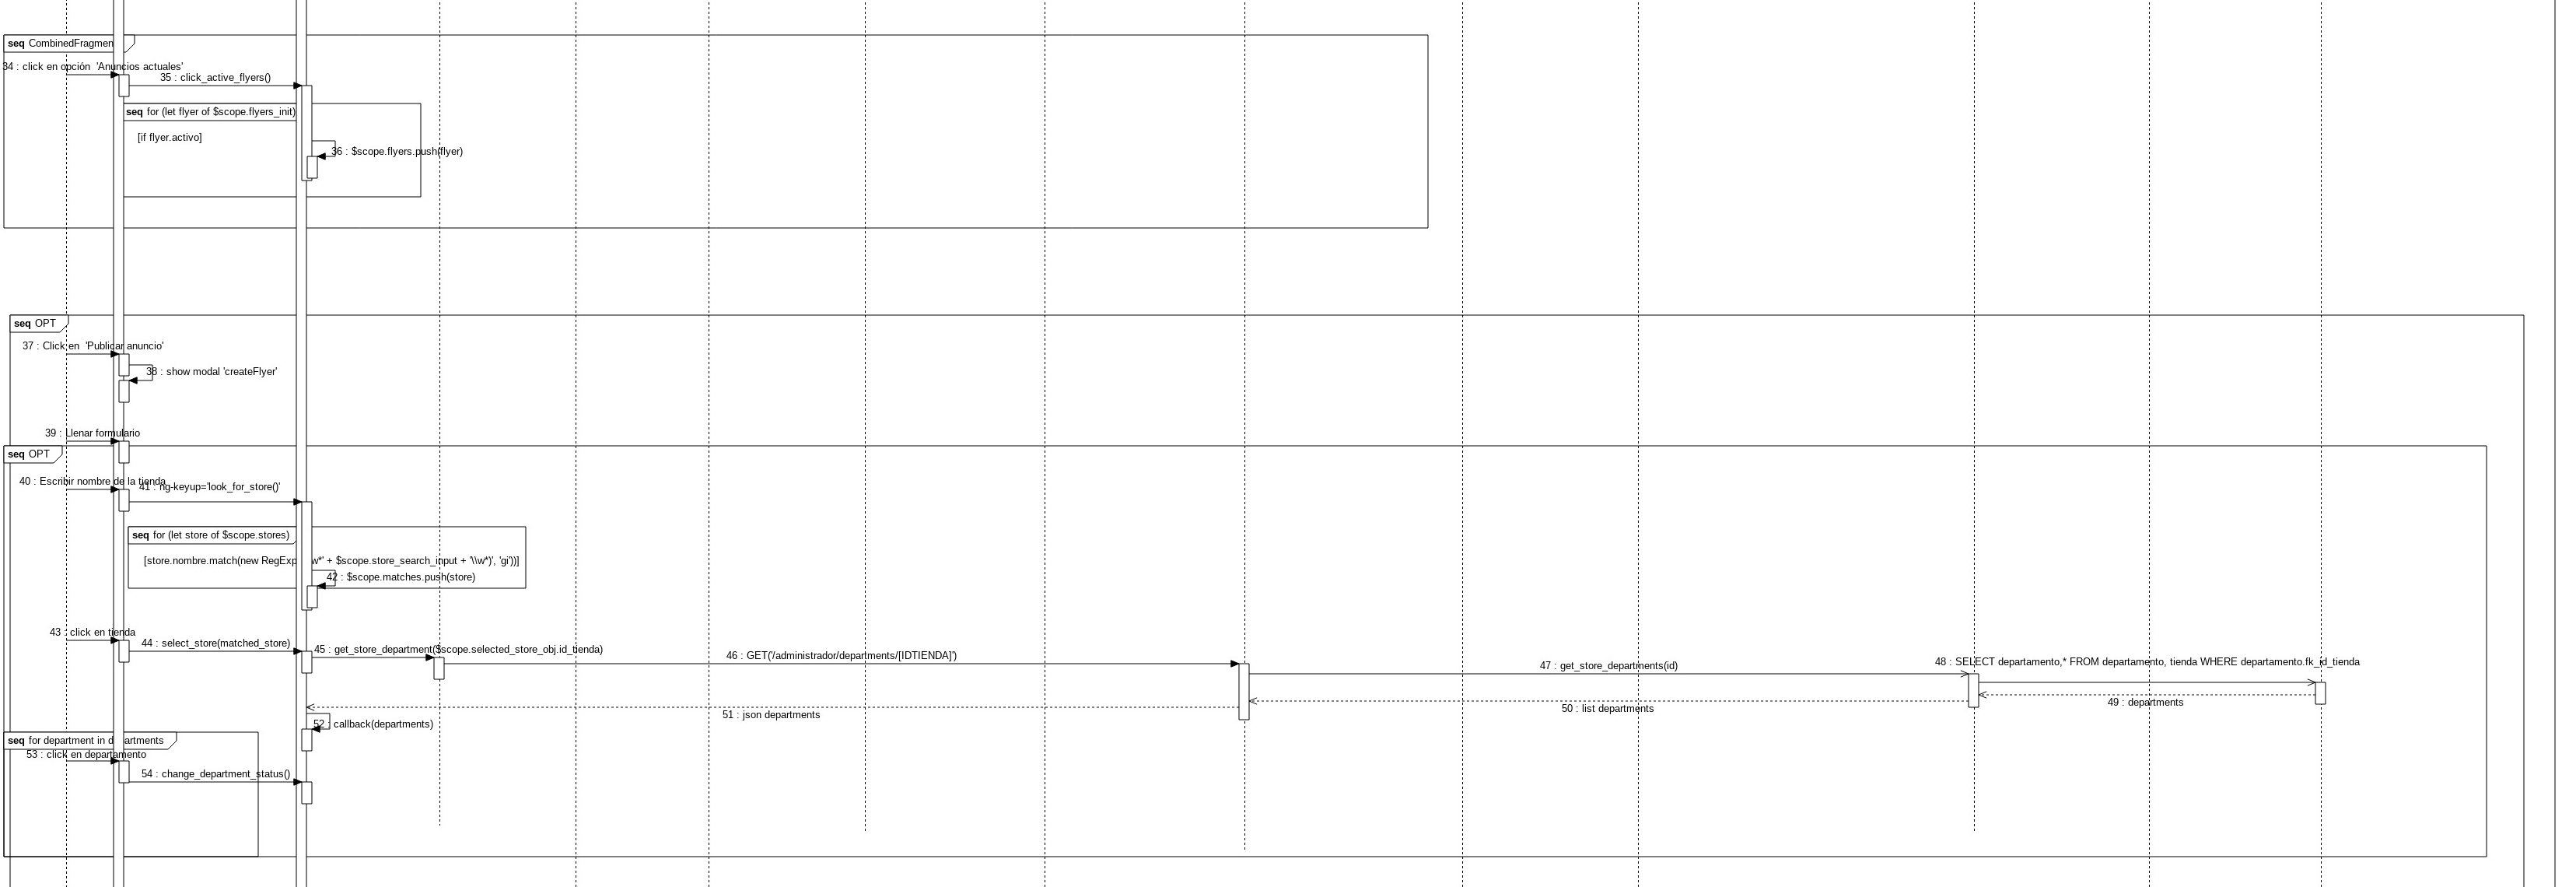
\includegraphics[width=1 \textwidth]{imagenes/DSRuben/anuncios3}
		\caption{Diagrama de secuencia Visualizar anuncios publicados (Parte 3).}
		\label{PADS:VisualizarAnuncio3}
\end{figure}
\FloatBarrier

\FloatBarrier
\begin{figure}[htbp!]
		\centering
			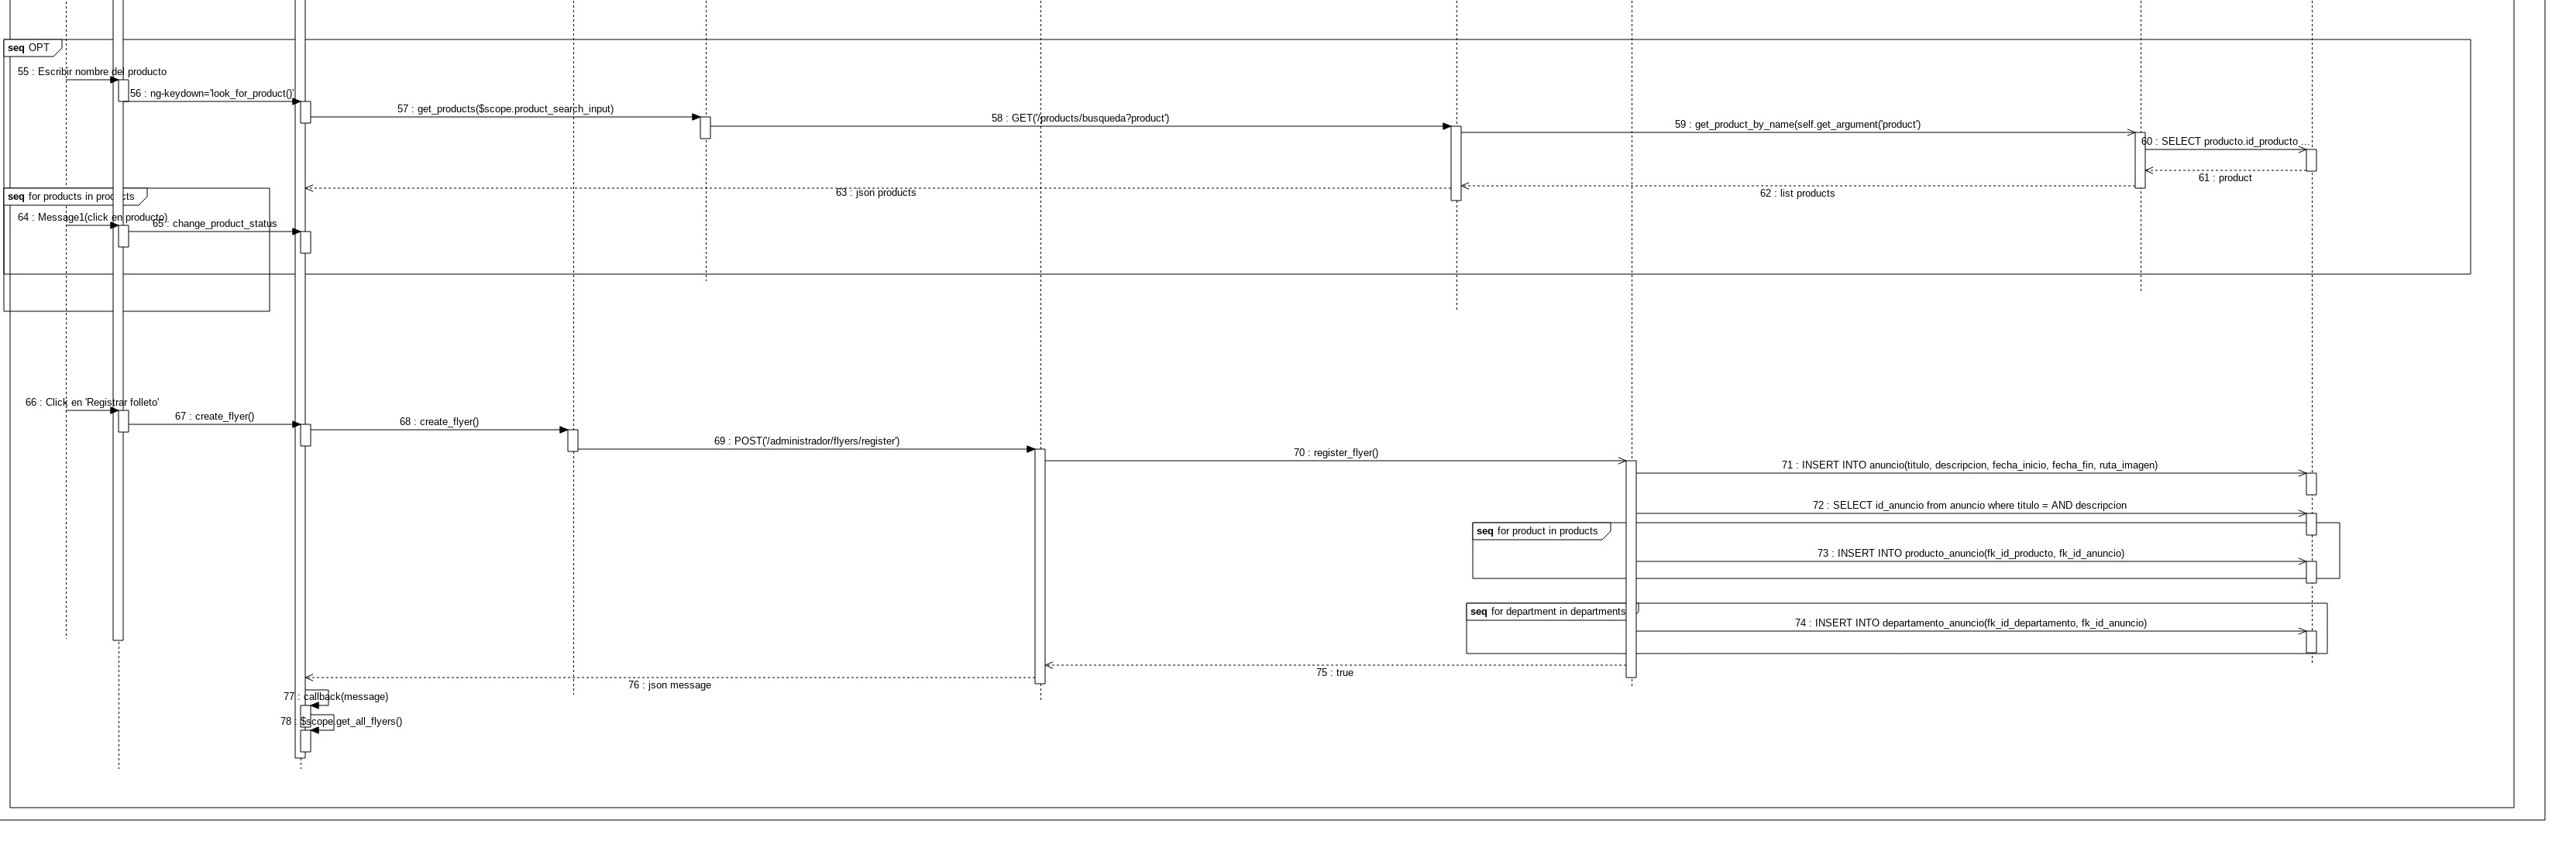
\includegraphics[width=1 \textwidth]{imagenes/DSRuben/anuncios4}
		\caption{Diagrama de secuencia Visualizar anuncios publicados (Parte 4).}
		\label{PADS:VisualizarAnuncio4}
\end{figure}
\FloatBarrier

La figura \ref{PADS:VisualizarBeacon} muestra el diagrama satisface el caso de uso \hyperlink{casosdeusoPA}{Visualizar Beacons registrados} que se muestra en el diagrama de casos de uso. \\
\textit{Notas:}
\begin{enumerate}
\item \textit{El diagrama fue separado en varias figuras para su visualización (Figura \ref{PADS:VisualizarBeacon}, Figura \ref{PADS:VisualizarBeacon2}, Figura \ref{PADS:VisualizarBeacon2}).}
\item \textit{Dentro del diagrama se encuentran también los casos de uso \hyperlink{casosdeusoPA}{Visualizar información de Beacon almacenada}, \hyperlink{casosdeusoPA}{Actualizar información de Beacon}.} 
\end{enumerate}

\FloatBarrier
\begin{figure}[htbp!]
		\centering
			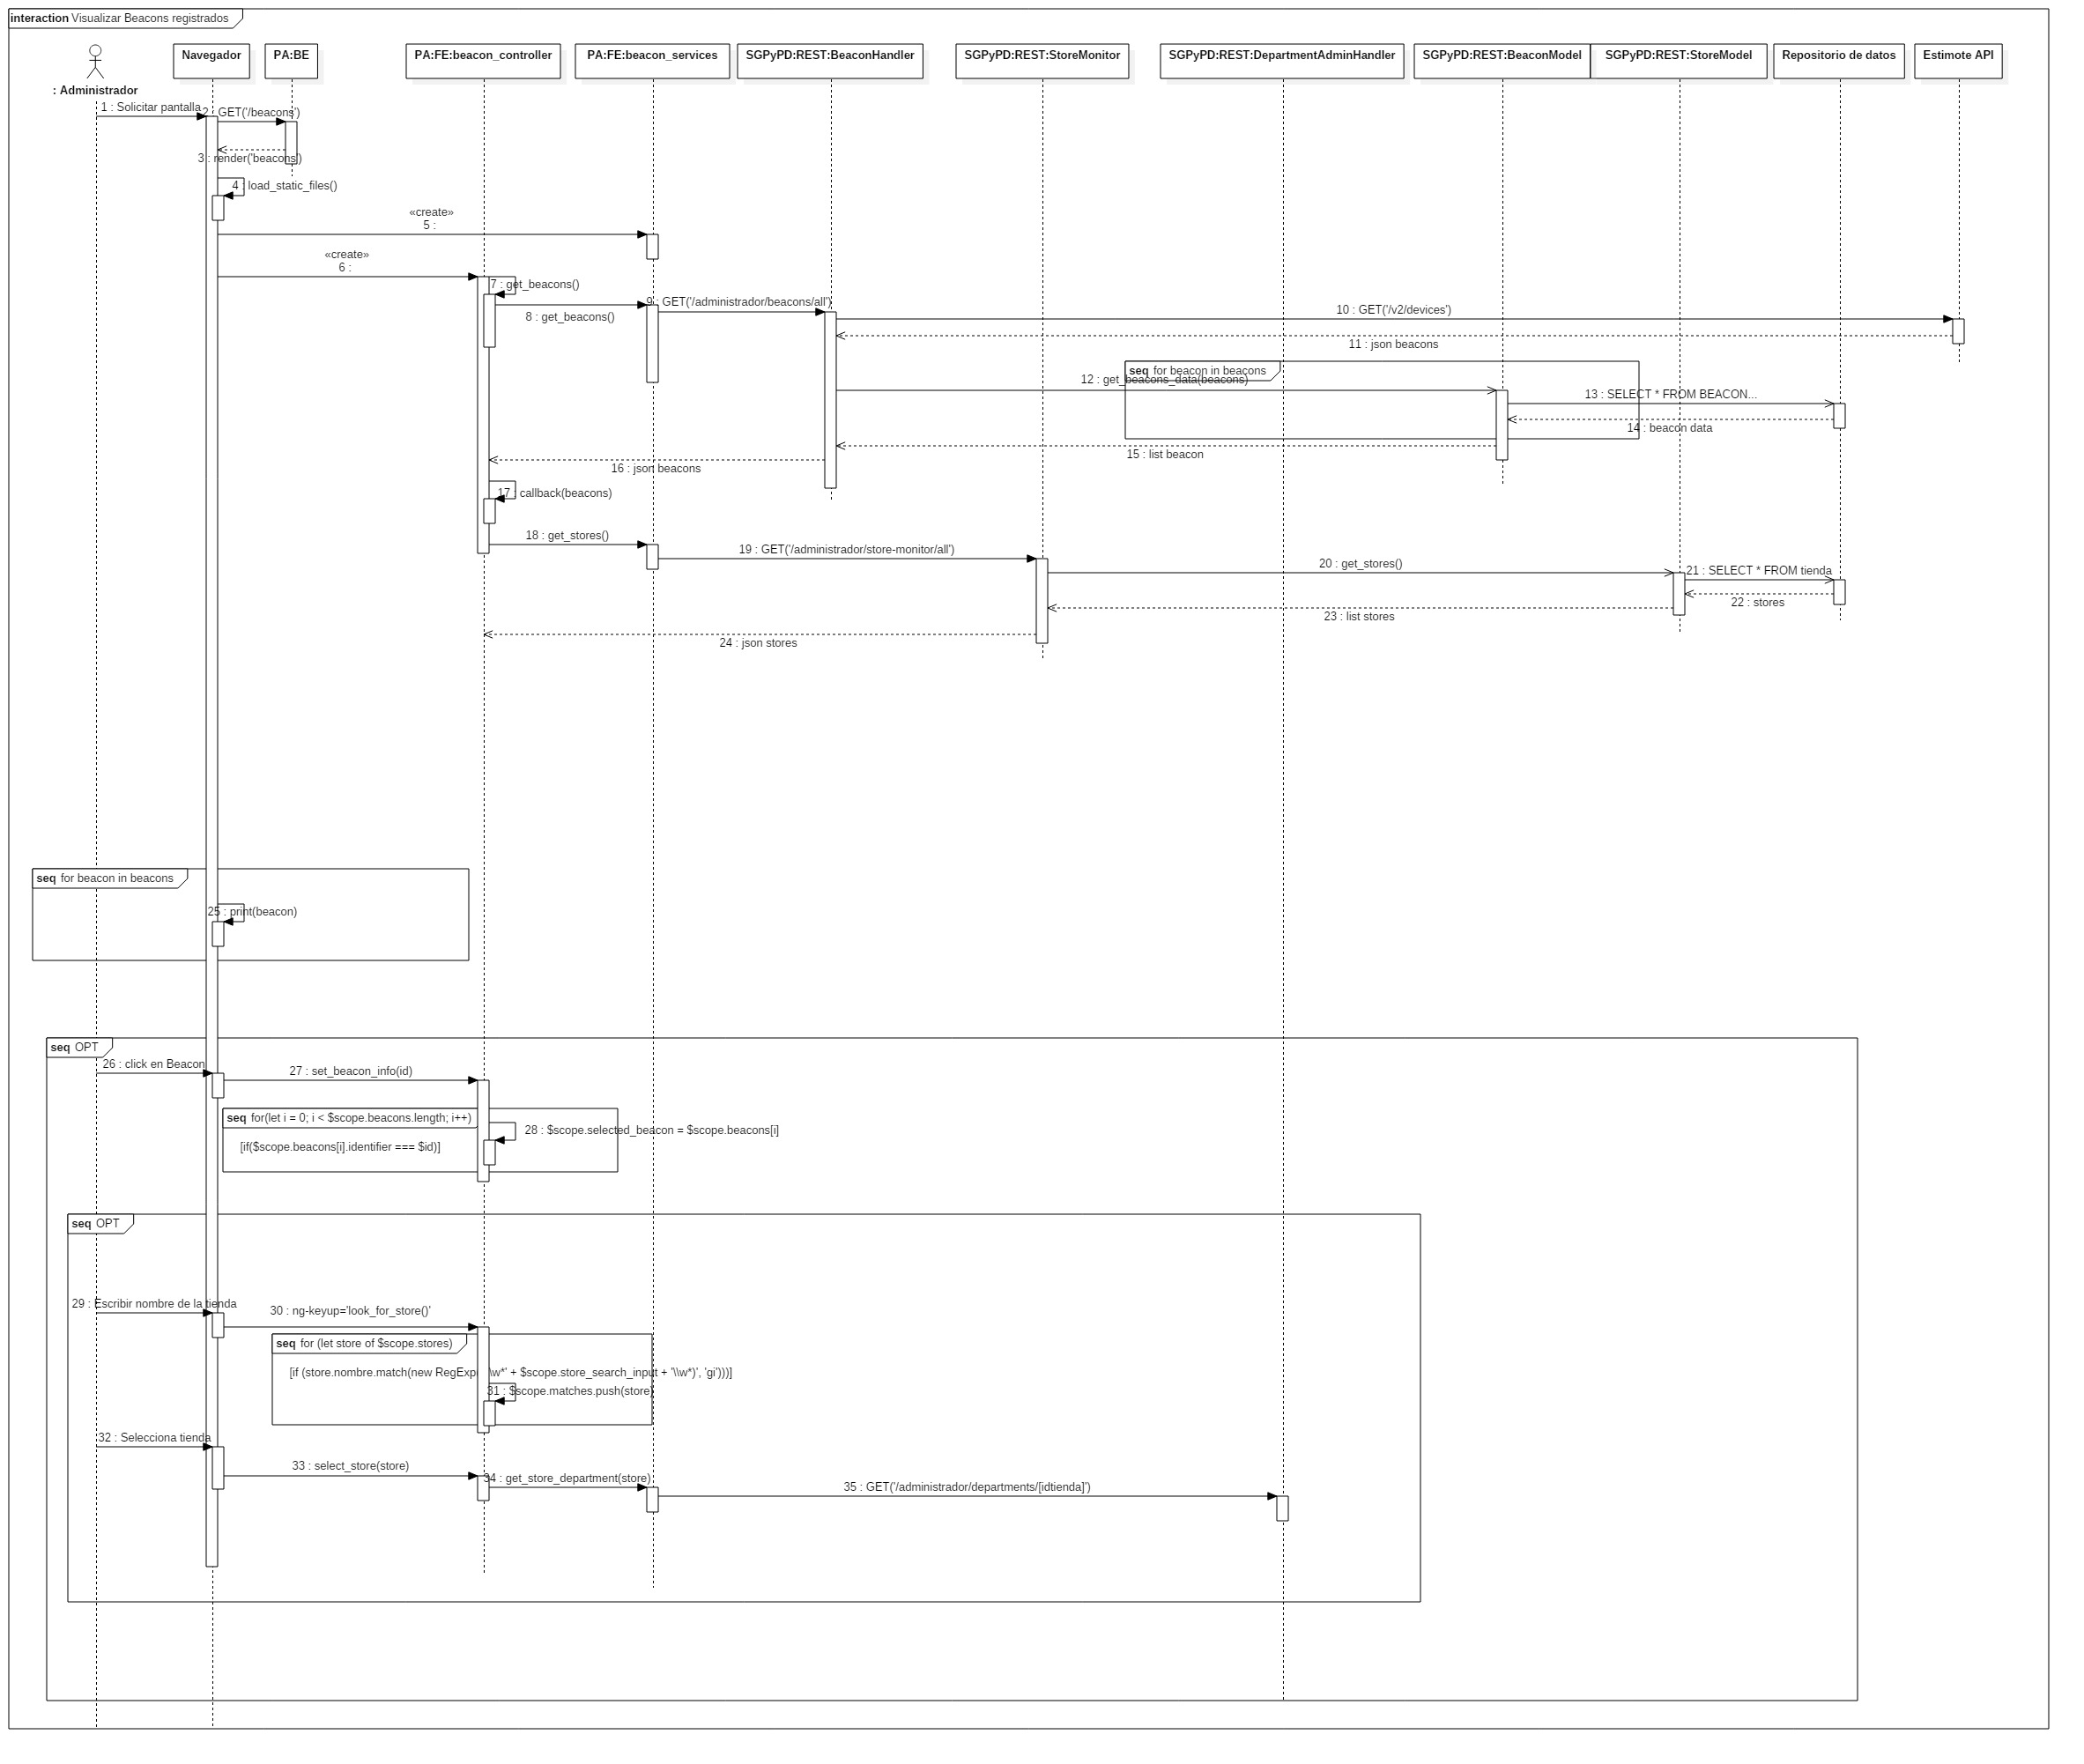
\includegraphics[width=1 \textwidth]{imagenes/DSRuben/beacons}
		\caption{Diagrama de secuencia Visualizar Beacons registrados (Visualización completa).}
		\label{PADS:VisualizarAnuncio}
\end{figure}
\FloatBarrier



\FloatBarrier
\begin{figure}[htbp!]
		\centering
			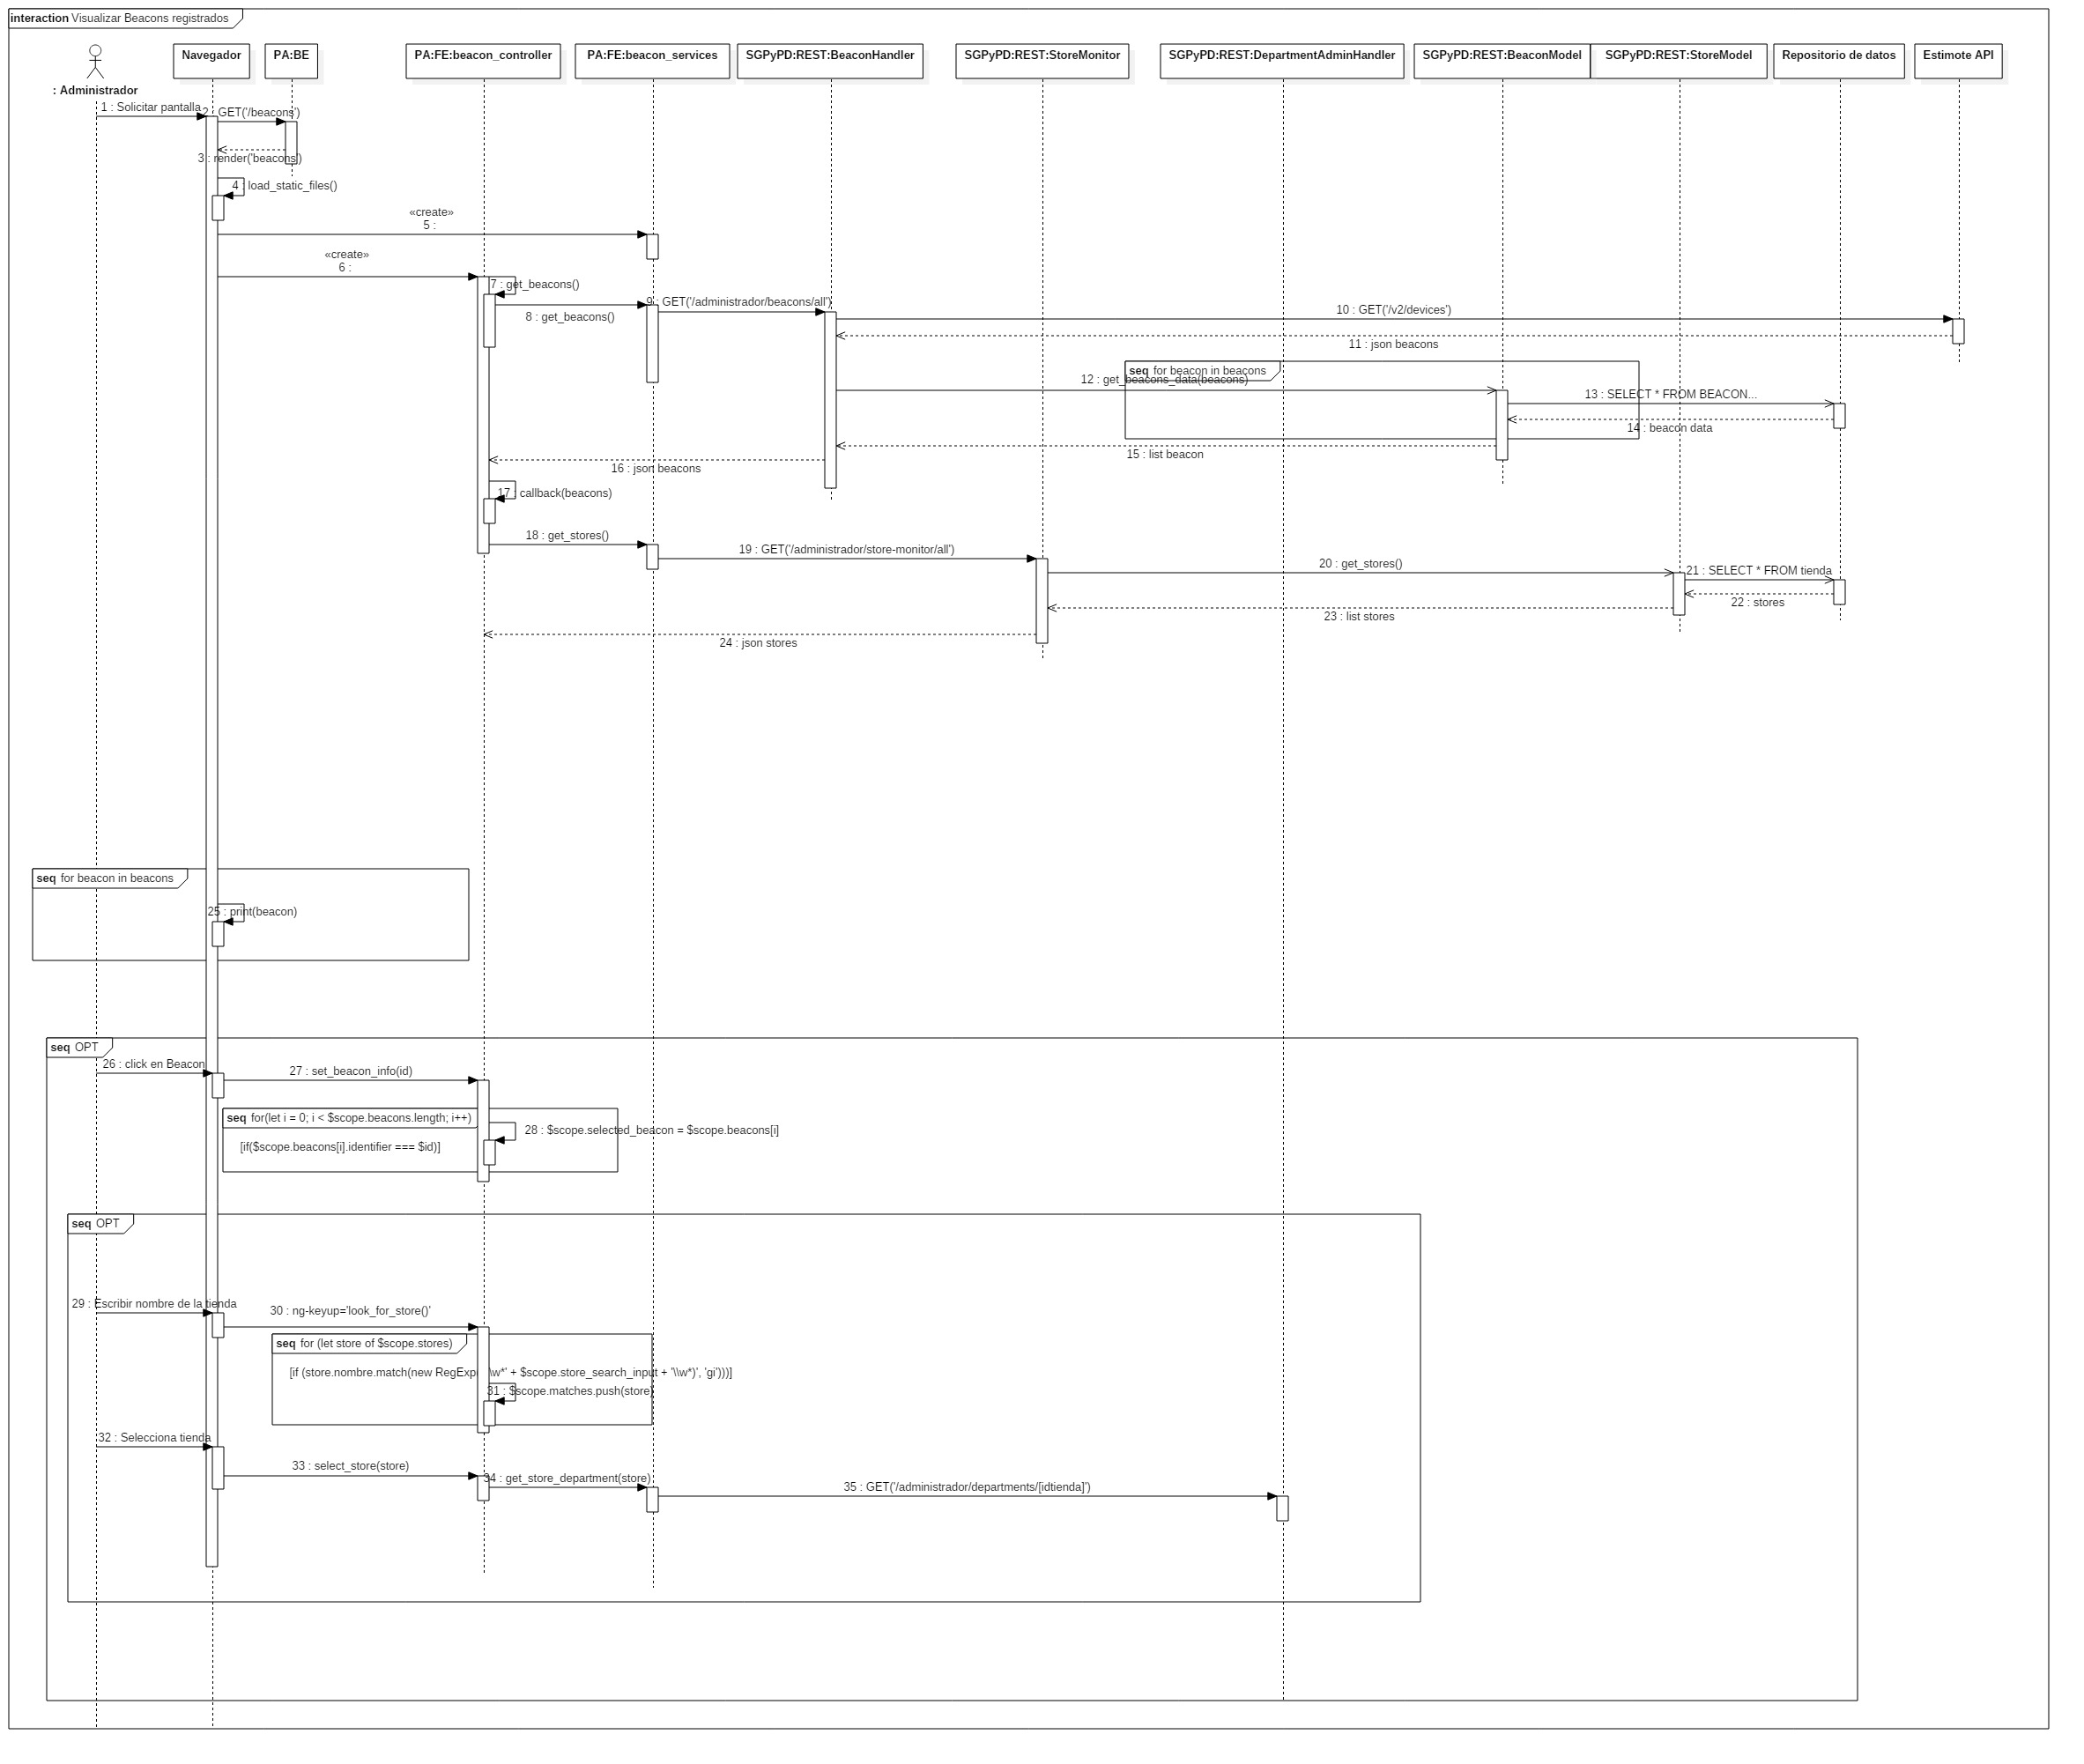
\includegraphics[width=1 \textwidth]{imagenes/DSRuben/beacons}
		\caption{Diagrama de secuencia Visualizar Beacons registrados (Visualización completa).}
		\label{PADS:VisualizarBeacon}
\end{figure}
\FloatBarrier

\FloatBarrier
\begin{figure}[htbp!]
		\centering
			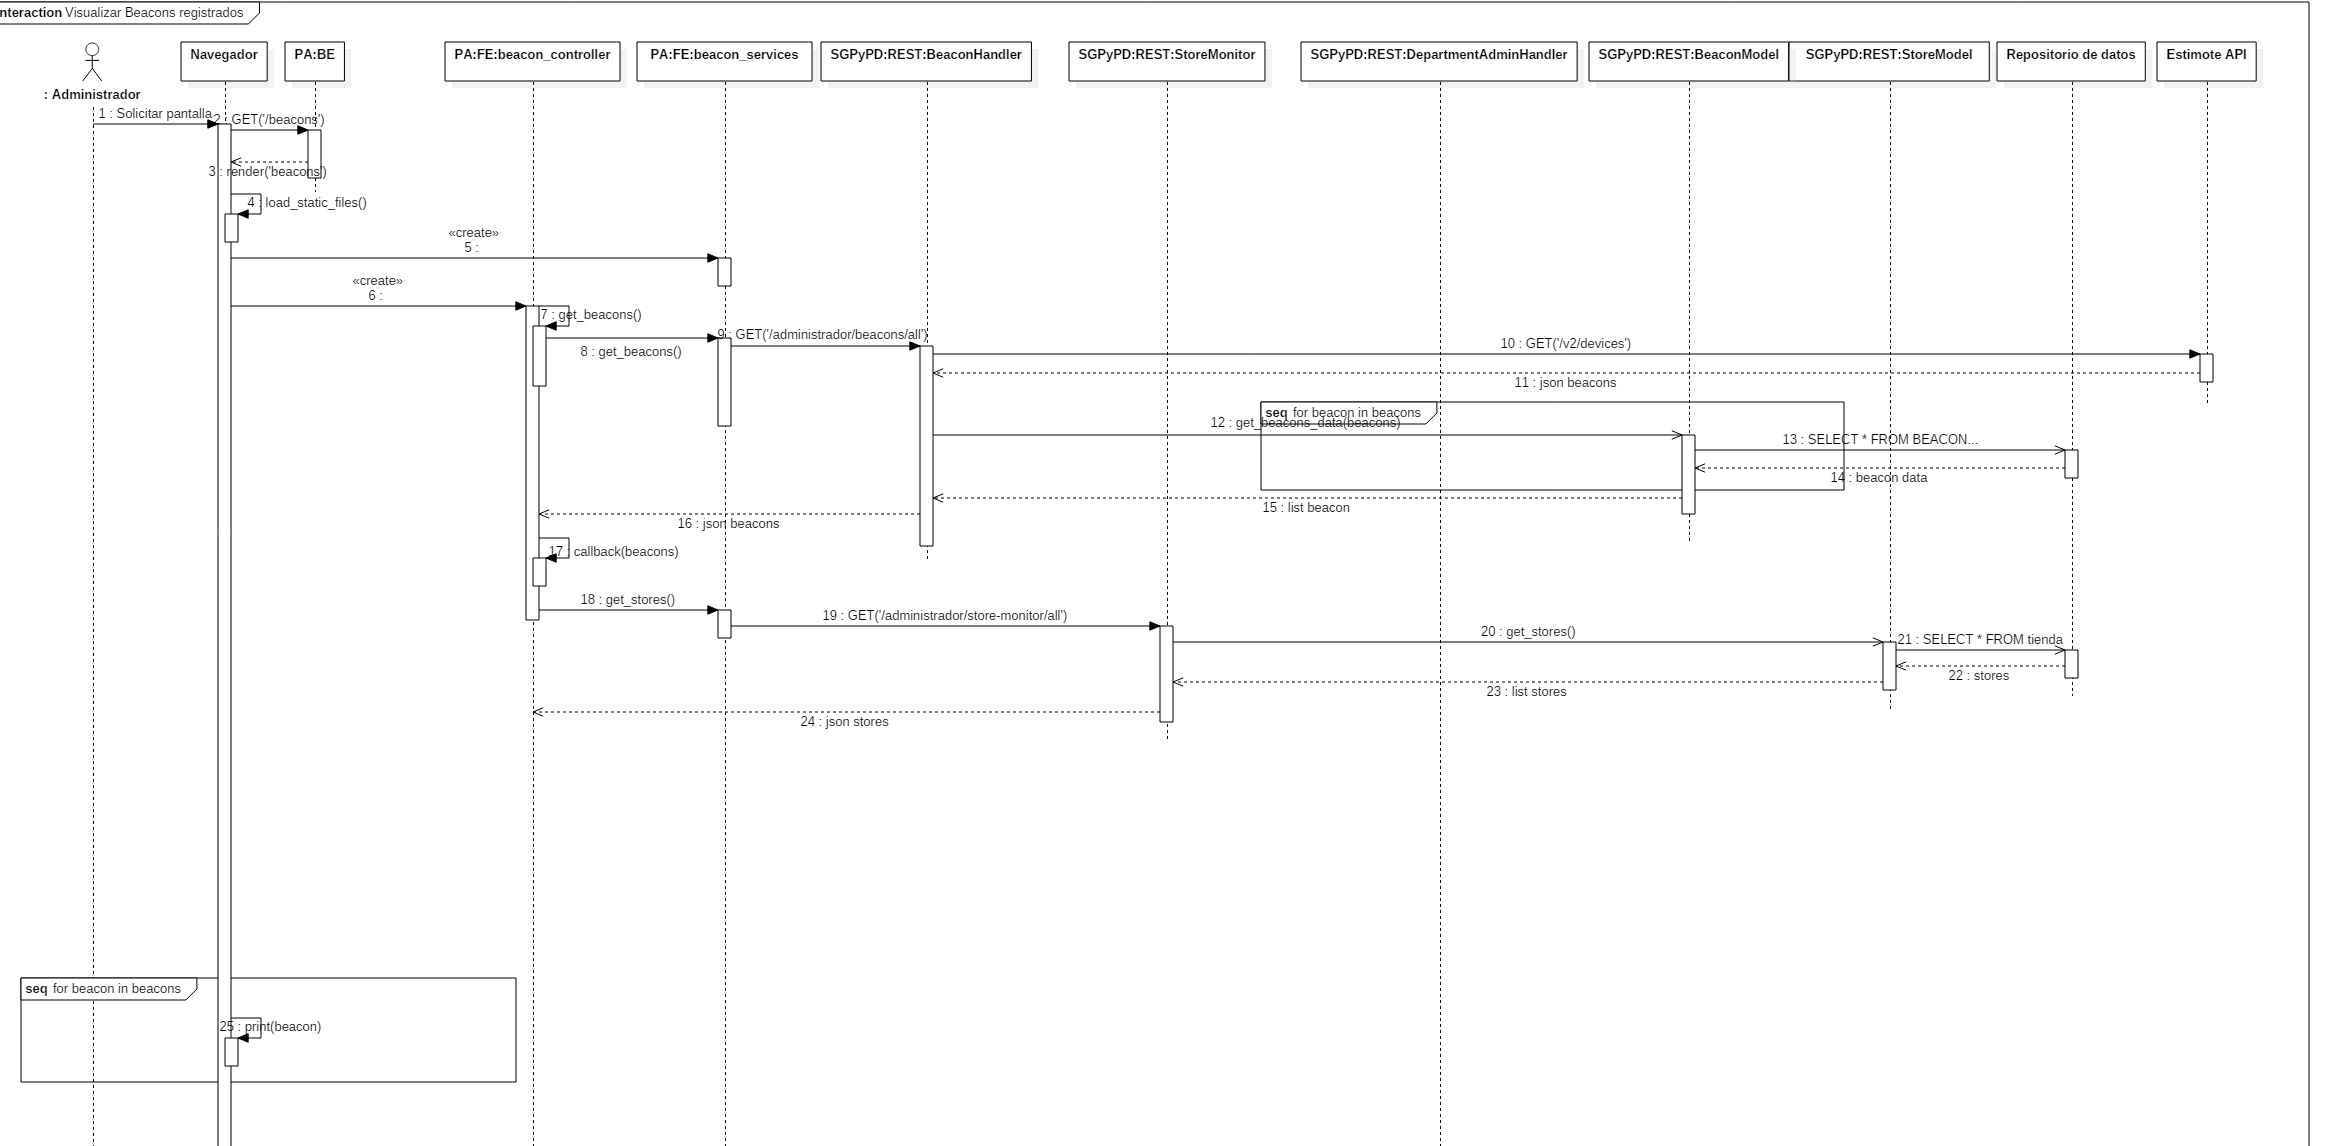
\includegraphics[width=1 \textwidth]{imagenes/DSRuben/beacons1}
		\caption{Diagrama de secuencia Visualizar Beacons registrados (Parte 1).}
		\label{PADS:VisualizarBeacon1}
\end{figure}
\FloatBarrier

\FloatBarrier
\begin{figure}[htbp!]
		\centering
			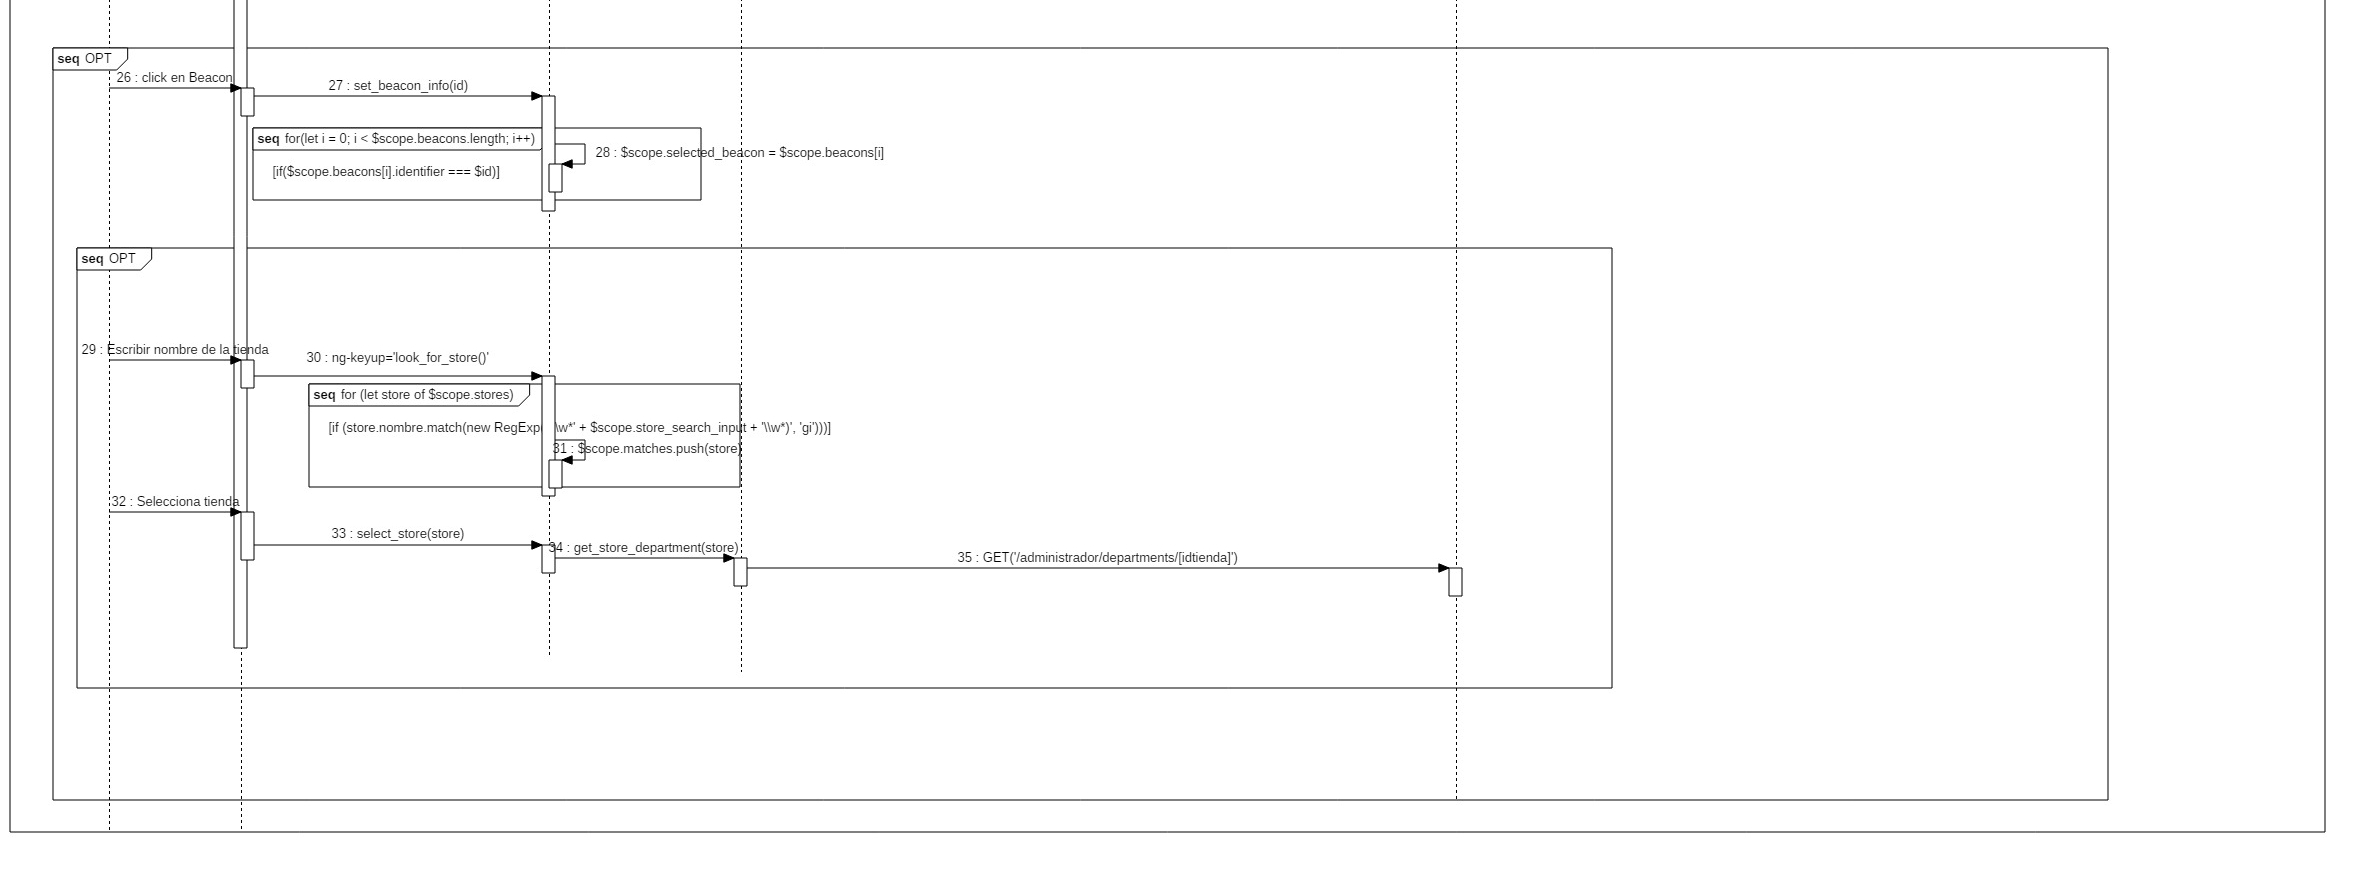
\includegraphics[width=1 \textwidth]{imagenes/DSRuben/beacons2}
		\caption{Diagrama de secuencia Visualizar Beacons registrados (Parte 2).}
		\label{PADS:VisualizarBeacon2}
\end{figure}
\FloatBarrier

%%% INTERFAZ DE USUARIO 
\title{\textbf{Diseño de interfaz de usuario \\}}

En la Figura \ref{PA:iniciarsesion} se muestra la interfaz de usuario que satisface el requerimiento \hyperlink{RFPA}{Iniciar sesión}.
\FloatBarrier
\begin{figure}[htbp!]
		\centering
			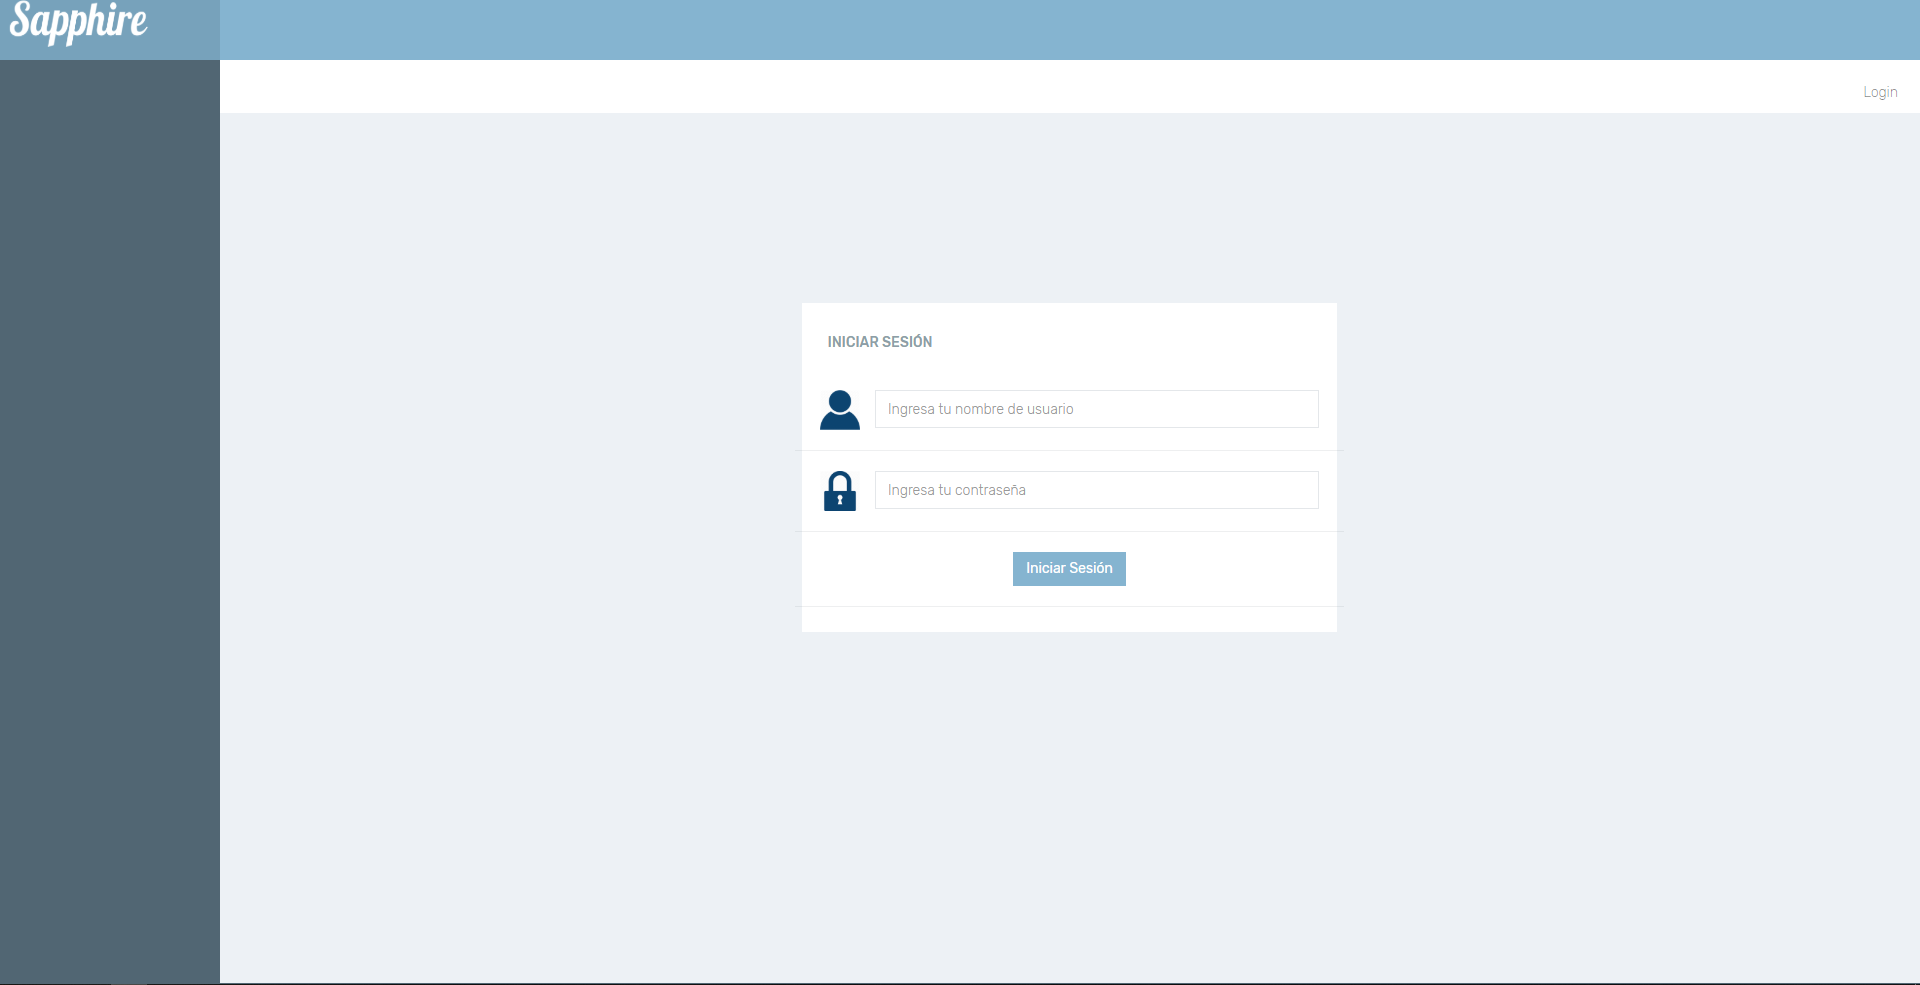
\includegraphics[width=1 \textwidth]{imagenes/UI/prototipo3/iniciarsesion}
		\caption{UIPanel31: Iniciar sesión.}
		\label{PA:iniciarsesion}
\end{figure}
\FloatBarrier

En la Figura \ref{PA:anunciospublicados} se muestra la interfaz de usuario que satisface el requerimiento \hyperlink{RFPA}{Visualizar información de anuncios publicados}.
\FloatBarrier
\begin{figure}[htbp!]
		\centering
			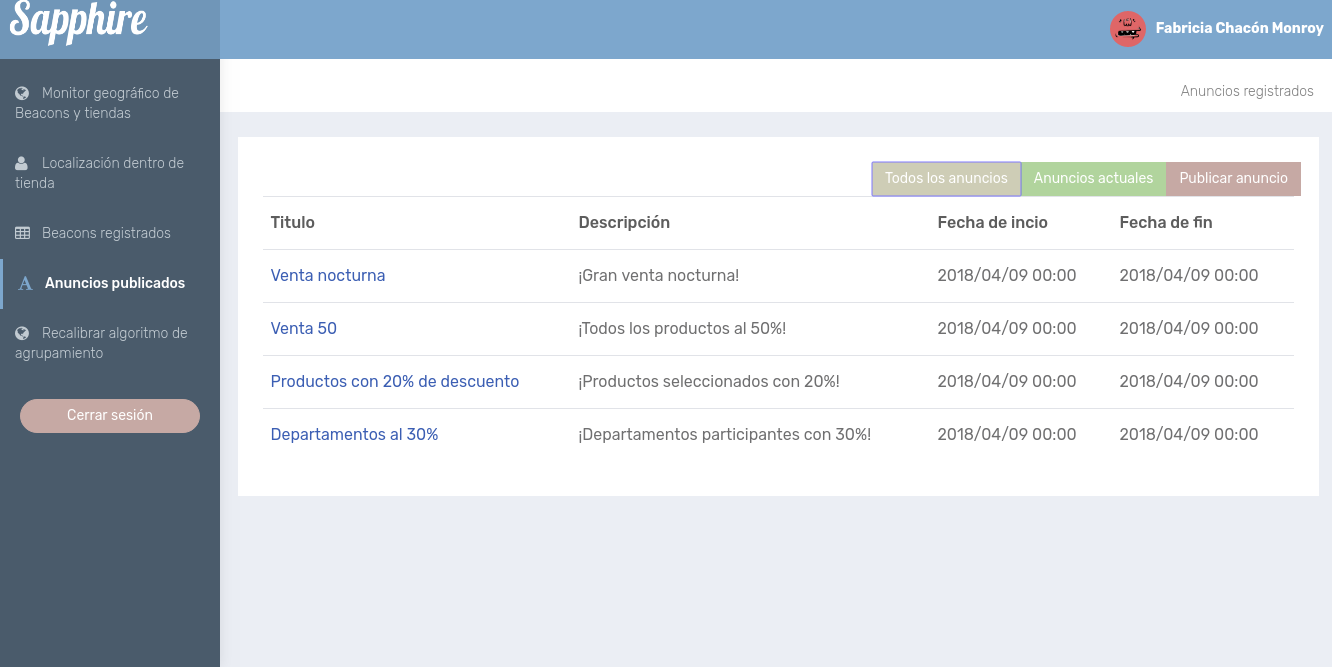
\includegraphics[width=1 \textwidth]{imagenes/UI/prototipo3/anunciosregistrados}
		\caption{UIPanel32: Anuncios publicados.}
		\label{PA:anunciospublicados}
\end{figure}
\FloatBarrier

En la Figura \ref{PA:anunciospublicados2} se muestra la pantalla que muestra la información detallada de un anuncio que satisface el requerimiento \hyperlink{RFPA}{Visualizar información de anuncios publicados}.
\FloatBarrier
\begin{figure}[htbp!]
		\centering
			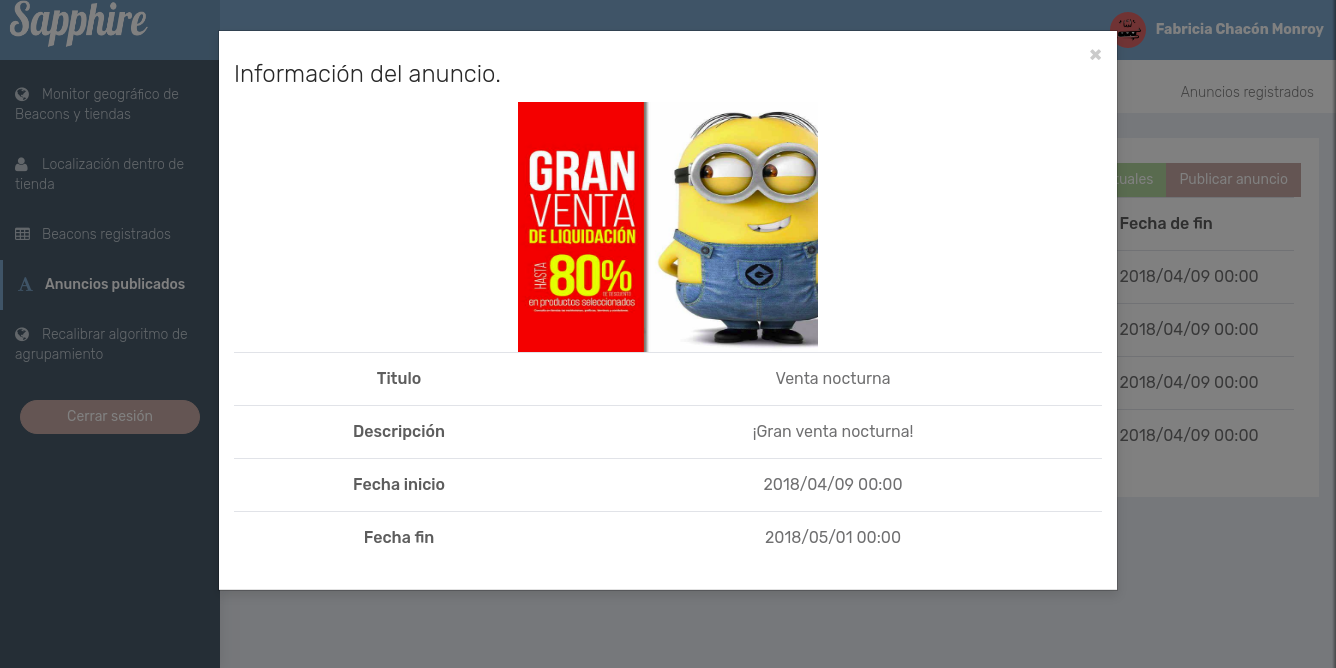
\includegraphics[width=1 \textwidth]{imagenes/UI/prototipo3/anunciosregistrados2}
		\caption{UIPanel33: Información específica de un anuncio.}
		\label{PA:anunciospublicados2}
\end{figure}
\FloatBarrier


En la Figura \ref{PA:anunciospublicados3} se muestra el formulario para registrar un nuevo anuncio que satisface el requerimiento \hyperlink{RFPA}{Visualizar información de anuncios publicados}.
\FloatBarrier
\begin{figure}[htbp!]
		\centering
			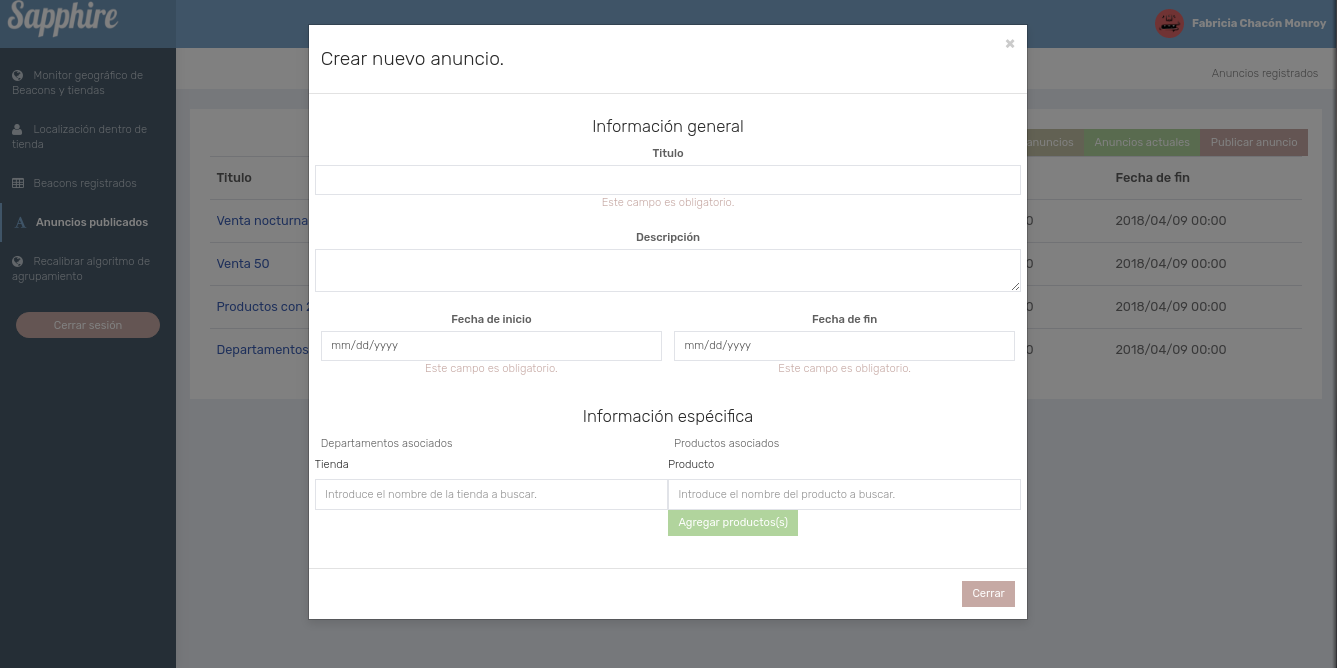
\includegraphics[width=1 \textwidth]{imagenes/UI/prototipo3/anunciosregistrados3}
		\caption{UIPanel34: Crear nuevo anuncio.}
		\label{PA:anunciospublicados3}
\end{figure}
\FloatBarrier



%%%%%%%%%%%%%%% BEACON

En la Figura \ref{PA:beacons1} se muestra la interfaz de usuario que satisface el requerimiento \hyperlink{RFPA}{Visualizar información de Beacons}.
\FloatBarrier
\begin{figure}[htbp!]
		\centering
			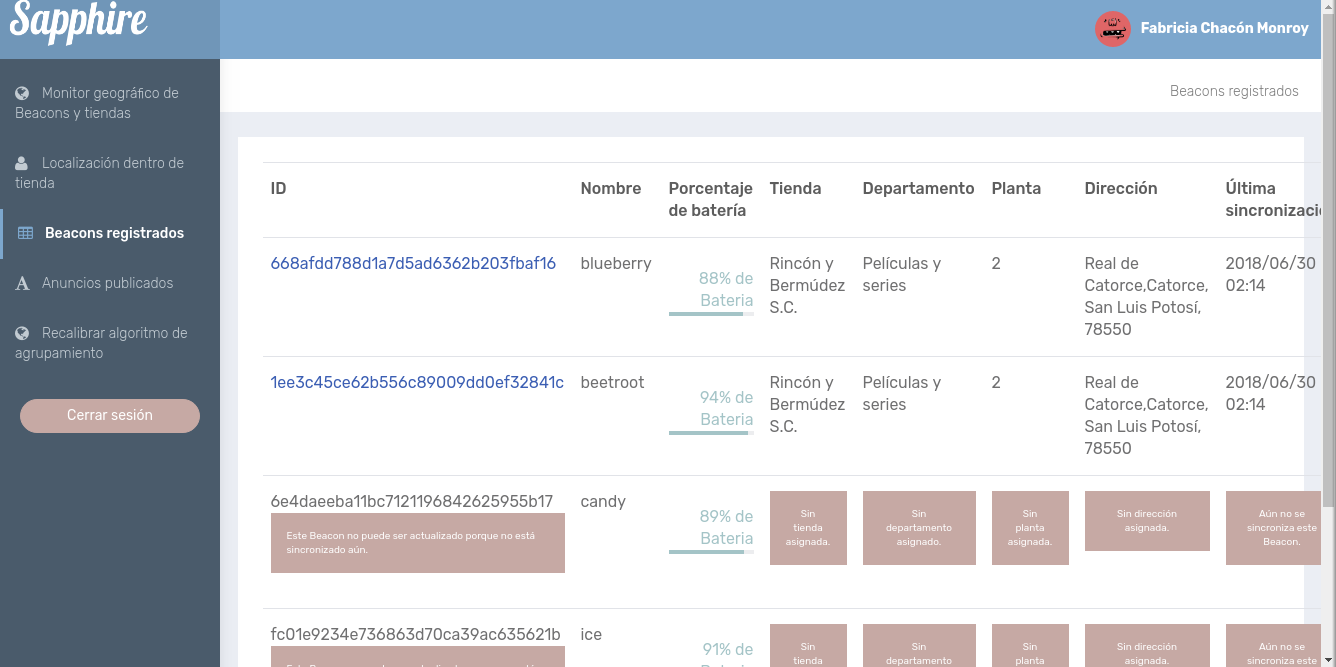
\includegraphics[width=1 \textwidth]{imagenes/UI/prototipo3/beacons1}
		\caption{UIPanel35: Visualizar Beacons.}
		\label{PA:beacons1}
\end{figure}
\FloatBarrier

En la Figura \ref{PA:beacons2} se muestra la pantalla que permite visualizar la información detallada de un Beacon y la posibilidad de modificar su información que satisface el requerimiento \hyperlink{RFPA}{Visualizar información de Beacons}.
\FloatBarrier
\begin{figure}[htbp!]
		\centering
			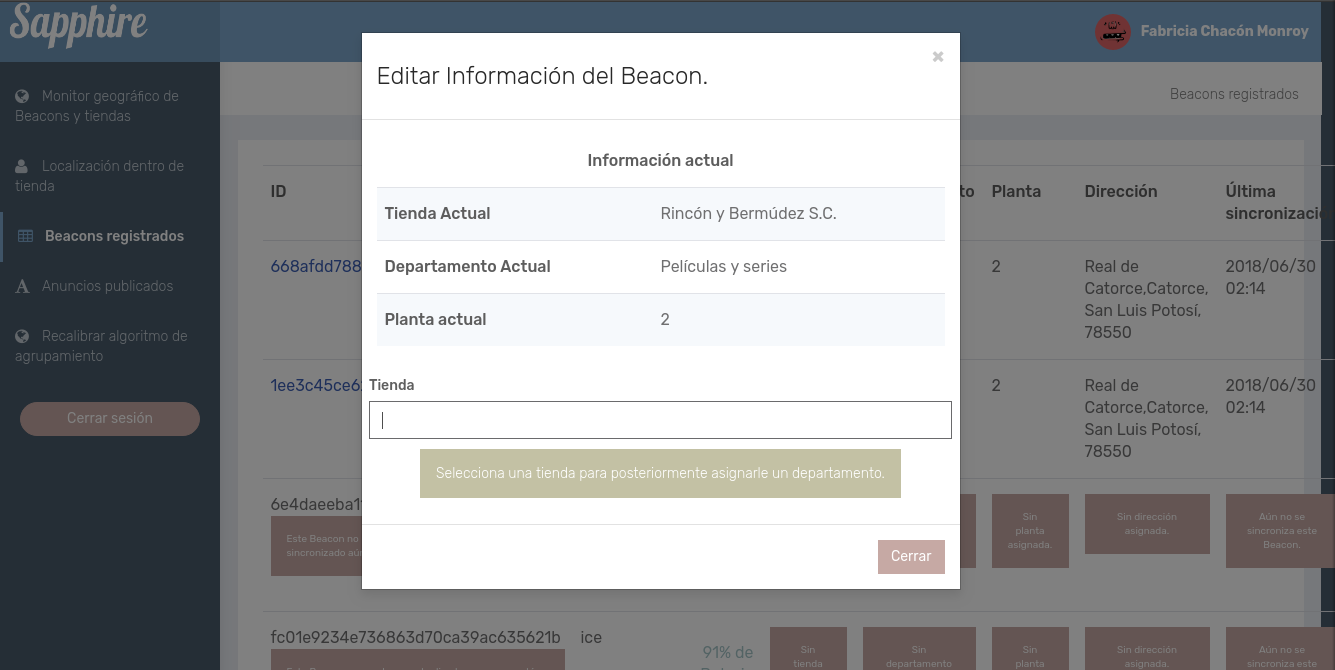
\includegraphics[width=1 \textwidth]{imagenes/UI/prototipo3/beacons2}
		\caption{UIPanel36: Información de Beacon específica.}
		\label{PA:beacons2}
\end{figure}
\FloatBarrier


\paragraph{Flujo de navegación del Panel de Administración.} ~\\

La figura \ref{PA:flujo4} muestra como es el flujo de navegación general del Panel de Admnistración.

\FloatBarrier
\begin{figure}[htbp!]
		\centering
			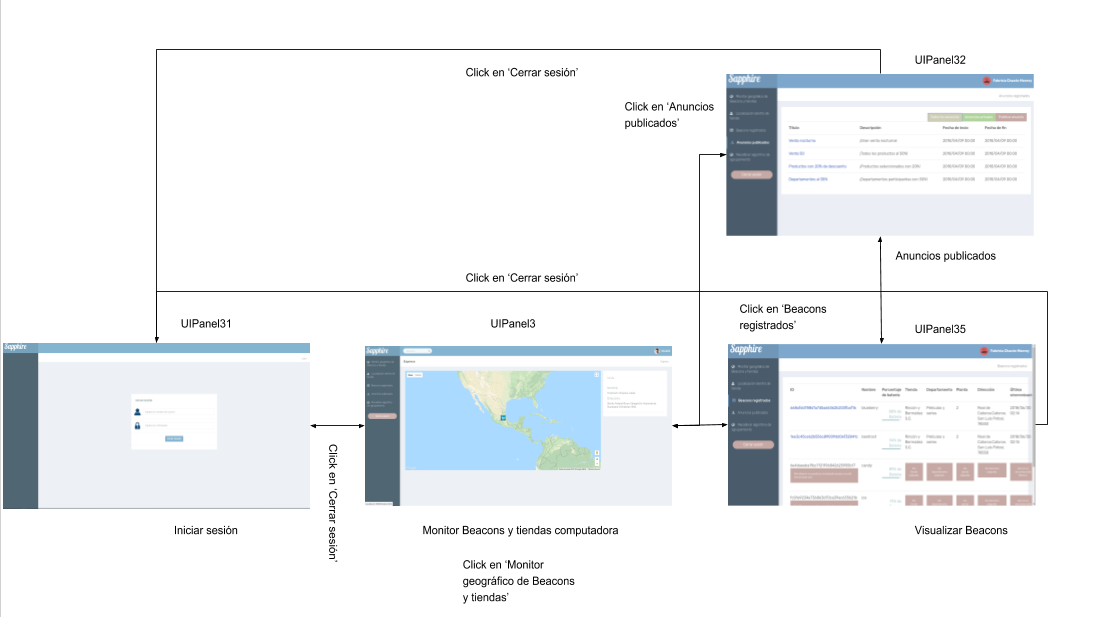
\includegraphics[width=1 \textwidth]{imagenes/paneladminmapa/general3}
		\caption{Flujo de navegación general Panel de Administración.}
		\label{PA:flujo4}
\end{figure}
\FloatBarrier



La figura \ref{PA:flujoBeacons} muestra como es el flujo de navegación de la pantalla \textbf{Beacons registrados}.

\FloatBarrier
\begin{figure}[htbp!]
		\centering
			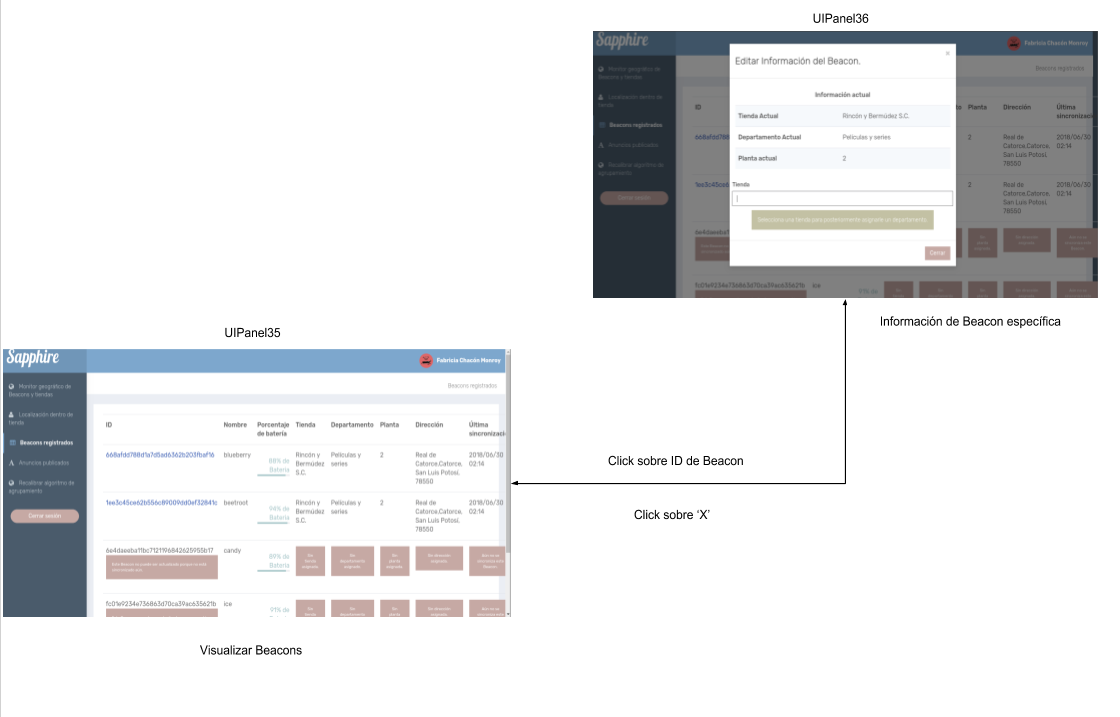
\includegraphics[width=1 \textwidth]{imagenes/paneladminmapa/beacons3}
		\caption{Flujo de navegación de pantalla Beacons registrados.}
		\label{PA:flujoBeacons}
\end{figure}
\FloatBarrier

La figura \ref{PA:flujoBeacons} muestra como es el flujo de navegación de la pantalla \textbf{Anuncios publicados}.

\FloatBarrier
\begin{figure}[htbp!]
		\centering
			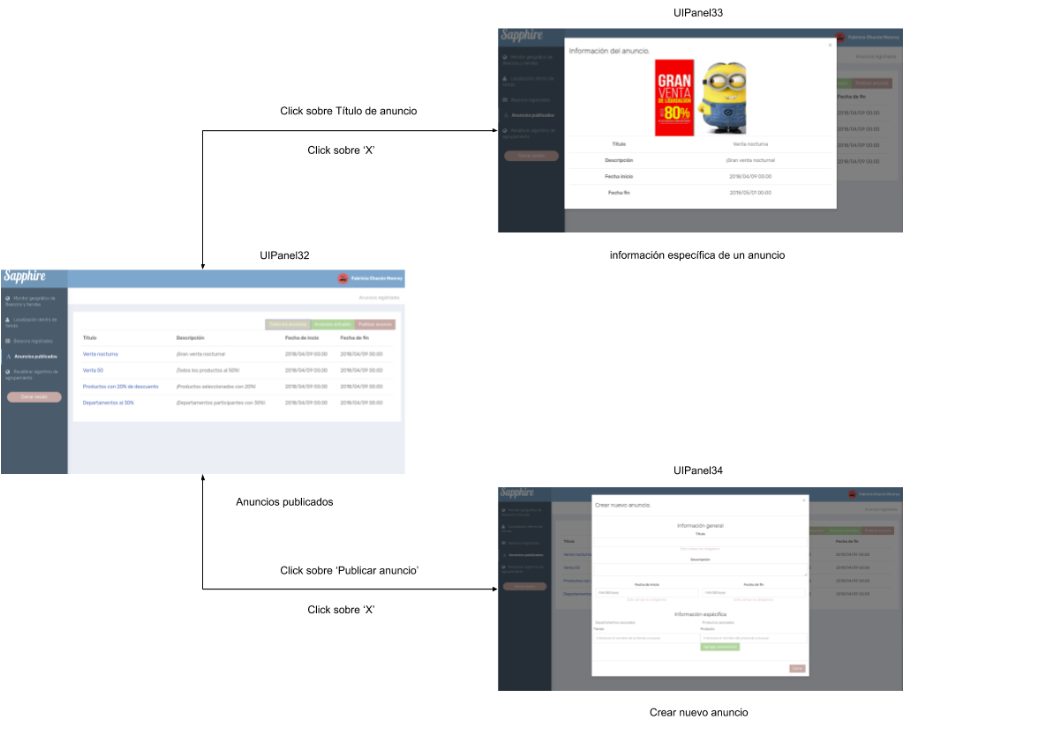
\includegraphics[width=1 \textwidth]{imagenes/paneladminmapa/anuncios3}
		\caption{Flujo de navegación de pantalla Anuncios publicados.}
		\label{PA:flujoAnuncios}
\end{figure}
\FloatBarrier

